\documentclass[a4paper,12pt]{article}
\usepackage{titlesec}

%cv rajo dependance 
\usepackage[left=1.5cm,right=1.5cm,top=1.5cm,bottom=1.5cm]{geometry}
\usepackage{graphicx}
\usepackage{parskip}
\usepackage{enumitem}
\usepackage{titlesec}
\usepackage{float} 
\usepackage{multicol}
\usepackage{helvet}
\usepackage{xcolor}
\usepackage[skins]{tcolorbox}
\renewcommand{\familydefault}{\sfdefault}

% Couleurs modernes
\definecolor{accentcolor}{RGB}{44,62,80}
\definecolor{secondarycolor}{RGB}{52,152,219}

% Ajustement des espacements
\setlength{\parskip}{4pt}
\setlength{\itemsep}{2pt}

% Titres des sections avec style moderne
\titleformat{\section}{\color{accentcolor}\large\bfseries\uppercase}{}{0em}{}[\titlerule]

% Style pour les compétences
\newtcolorbox{skillbox}{colback=white, colframe=secondarycolor!20, arc=3pt, boxsep=3pt, left=4pt, right=4pt}

% fin cv rajo



% vo ni-ajouterna
\usepackage{booktabs}
\usepackage{array}
\usepackage{tabularx}
\usepackage{longtable}
\usepackage{colortbl}
\usepackage{xcolor}
\usepackage{pgfplots}
\usepackage{tikz}
\usetikzlibrary{positioning}
\pgfplotsset{compat=1.17}
% Définition des couleurs pour les catégories
\definecolor{electronique}{RGB}{70,130,180}
\definecolor{vetements}{RGB}{255,69,0}
\definecolor{maison}{RGB}{34,139,34}
\definecolor{sports}{RGB}{255,215,0}
\definecolor{alimentaire}{RGB}{220,20,60}
\definecolor{beaute}{RGB}{186,85,211}

%fin vo ni-ajouterna

\usepackage{shorttoc} % pour générer un sommaire allégé

\titleformat{\chapter}[hang] % 'hang' évite le retour à la ligne
  {\normalfont\huge\bfseries} % style
  {Chapitre \thechapter :} % numéro avec texte
  {1em} % espace entre numéro et titre
  {} % code avant le titre

\usepackage[utf8]{inputenc}

\usepackage{caption} % à mettre dans le préambule
\usepackage{url}  % Pour utiliser \url{...} dans les références
\usepackage{pdfpages}
\usepackage{graphicx} % à mettre dans le préambule

\definecolor{monbleu}{RGB}{0,0,255} % bleu pur RGB
\definecolor{bleuciel}{RGB}{90,170,210} % bleu ciel

\usepackage{graphicx} % Pour insérer des images
\usepackage{geometry}
\usepackage{setspace} % Pour gérer l'interligne
\usepackage{xcolor}
\usepackage{tcolorbox}
\usepackage{float}
\usepackage[T1]{fontenc} 
\usepackage{newtxtext} % Texte en Times New Roman
\usepackage{newtxmath} % Symboles mathématiques compatibles Times


%packages pour ajouter le code python 
\usepackage{listings}
\usepackage{xcolor} % déjà présent, utile pour les couleurs dans le code

\geometry{margin=2.5cm}


% Définition du style pour le code Python
\lstdefinestyle{pythonstyle}{
    language=Python,
    basicstyle=\ttfamily\small,
    keywordstyle=\color{blue}\bfseries,
    commentstyle=\color{gray}\itshape,
    stringstyle=\color{red},
    numbers=left,
    numberstyle=\tiny,
    stepnumber=1,
    numbersep=5pt,
    showstringspaces=false,
    breaklines=true,
    frame=single,
    captionpos=b
}


\usepackage{titlesec}
\titlespacing*{\chapter}{0pt}{-20pt}{20pt}


\begin{document}

% ---------------- Page de garde personnalisée ----------------
\begin{titlepage}
    \thispagestyle{empty} % Pas de numéro de page
    \begin{center}
        
\includegraphics[width=6cm]{logo_insi.png} \\[0.5cm]
        {\textbf{\large INSI UNIVERSITY}} \\[0.5cm]

        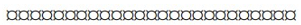
\includegraphics[width=6cm]{transition.png} \\[0.5cm]
        \textbf{INSTITUT NATIONAL SUPERIEUR D’INFORMATIQUE} \\[1cm]

        \textit{\textbf{Domaine :}} Sciences et Technologies \\
        \textit{\textbf{Mention :}} Informatique \\
        \textit{\textbf{Parcours :}} Intelligence Artificielle \\[1cm]

        % Auteurs
        Par : \\
        \begin{tabular}[t]{@{}l@{}}
            Mademoiselle VOAHARIMPITIAVANA Andraina Faniriana \\
            Monsieur RAKOTONAVALONA Andriamihaingosoa Rajo Lalaina
        \end{tabular} \\[1cm]

        % Titre avec tcolorbox
        \begin{tcolorbox}[
            colback=bleuciel,   % couleur de fond
            colframe=blue!60,   % bordure
            arc=5mm,            % arrondi des coins
            boxrule=0pt,        % épaisseur de la bordure (ici invisible)
            left=10pt,          % marge intérieure gauche
            right=10pt,         % marge intérieure droite
            top=8pt,            % marge intérieure haut
            bottom=8pt,         % marge intérieure bas
            width=0.8\textwidth, % largeur réduite
            center
        ]
        \centering
        \textbf{\large ANALYSE DES HABITUDES D'ACHAT \\ SUR UNE PLATEFORME E-COMMERCE }
        \end{tcolorbox} 
        \vspace{0.5cm}

        
   \begin{flushleft}
   % Commission d'examen
        Soutenu le 03 Septembre 2025, devant la Commission d’Examen composée de : \\[0.5cm]
        \begin{tabular}{@{}ll@{}}
            \textbf{Président :}   & Dr RAKOTOMANANJARA David Fitiana\\[0.5cm]
            \textbf{Examinateur :} & Monsieur RASOLOFOMANANA Tolotra Iarivony Nirina\\[0.5cm]
            \textbf{Encadreur :}   & Dr RANDRIANARISON Nomenjanahary Tsirilala \\[1.5cm]
        \end{tabular} \\[1cm]
\end{flushleft}
        \begin{flushright}
            Année universitaire : 2024 – 2025
        \end{flushright}

    \end{center}
\end{titlepage}

% ---------------- Début de la numérotation ----------------
\cleardoublepage


\cleardoublepage        % finit la page actuelle et commence une nouvelle page
\thispagestyle{empty}   % pas de numéro de page sur cette page
\mbox{}                 % contenu vide pour générer la page blanche
\cleardoublepage

\pagenumbering{roman} % Numérotation en chiffres romains minuscules
\setcounter{page}{1}  % Commence à i

\chapter*{Remerciements}
\addcontentsline{toc}{chapter}{Remerciements}
\vspace{1cm}

Nous adressons nos plus profonds remerciements :

- Au directeur de l'école, Monsieur ANDRIAMANJAKA RAMASONDRANO, pour nous avoir confié ce travail, pour son suivi, sa disponibilité, ses orientations et ses conseils précieux ;

- Au Docteur RANDRIANARISON Nomenjanahary Tsirilala, notre encadrant pour ce projet, qui nous a accueillis et guidés avec bienveillance tout au long de ce travail ;

- À nos familles et amis pour leur soutien inébranlable, leurs encouragements et leur compréhension tout au long de cette période d'étude ;

- À tous ceux qui, de près ou de loin, ont contribué à la réussite de ce travail.

Vous avez toute notre gratitude.

% ---------- RÉSUMÉ ----------
\chapter*{Résumé}
\addcontentsline{toc}{chapter}{Résumé}
\vspace{1cm}

Ce mémoire présente l'implémentation de techniques avancées d'analyse de données pour décrypter les habitudes d'achat et segmenter la clientèle d'une plateforme e-commerce pakistanaise. La segmentation comportementale des clients s'avère un levier stratégique déterminant pour appréhender finement leurs patterns d'achat, anticiper l'évolution de leurs besoins et optimiser l'expérience d'achat sur le marché digital pakistanais en forte croissance.

L'étude s'appuie sur l'analyse approfondie de jeux de données transactionnelles exhaustifs (produits acquis, fréquence des commandes, valeur du panier moyen) afin de regrouper les clients en segments homogènes selon leurs comportements d'achat distinctifs. Cette segmentation multidimensionnelle permet la personnalisation des offres promotionnelles et le ciblage précis des actions marketing, favorisant ainsi la fidélisation à long terme de la clientèle et l'augmentation soutenue du chiffre d'affaires.

Les récents progrès des algorithmes de clustering (K-Means, DBSCAN) ont considérablement renforcé la pertinence opérationnelle des modèles de segmentation client dans l'écosystème du commerce électronique moderne.

À travers l'analyse comparative d'algorithmes de clustering et l'étude détaillée des paniers d'achat, cette recherche démontre comment une plateforme e-commerce pakistanaise peut exploiter l'analyse prédictive pour approfondir sa connaissance client et optimiser ses stratégies marketing dans un contexte concurrentiel dynamique.

\textbf{Mots-clés :} Analyse de données, Segmentation client, RFM, Clustering, Marketing digital, E-commerce, Basket Analysis, Marché pakistanais.

\vspace{1cm}
{\LARGE
\textbf{Abstract}}\\

This thesis explores the implementation of advanced data analysis techniques to decipher purchasing habits and segment the customer base of a Pakistani e-commerce platform. Behavioral customer segmentation proves to be a strategic lever for precisely understanding purchase patterns, anticipating evolving needs, and optimizing the shopping experience within Pakistan's rapidly growing digital market.

The study is based on comprehensive analysis of extensive transactional datasets (products purchased, order frequency, average basket value) to group customers into homogeneous segments according to their distinctive purchasing behaviors. This multidimensional segmentation enables the personalization of promotional offers and precise targeting of marketing actions, thereby fostering long-term customer loyalty and sustained revenue growth.

Recent advances in clustering algorithms (K-Means, DBSCAN) have significantly enhanced the operational relevance of customer segmentation models within the modern e-commerce ecosystem.

Through comparative analysis of clustering algorithms and detailed basket analysis, this research demonstrates how a Pakistani e-commerce platform can leverage predictive analytics to deepen customer understanding and optimize marketing strategies in a dynamic competitive landscape.

\textbf{Keywords:} Data Analysis, Customer Segmentation, RFM, Clustering, Digital Marketing, E-commerce, Basket Analysis, Pakistani Market.
% Début du sommaire
\chapter*{SOMMAIRE}
\vspace{0.5cm}
{\large
\textbf{REMERCIEMENTS}\par

\vspace{0.25cm}
\textbf{RÉSUMÉ}\par

\vspace{0.25cm}
\textbf{LISTE DES ABREVIATIONS}\par

\vspace{0.25cm}
\textbf{INTRODUCTION}\par

\vspace{0.25cm}
\textbf{CONCEPTION DU PROJET}\par

\vspace{0.5cm}

\hspace*{1.3cm}\textbf{I. PRÉSENTATION GÉNÉRALE}\par
\hspace*{1.8cm}I.1. Présentation de l’INSI\par
\hspace*{1.8cm}I.2. Cadre théorique et revue de littérature\par

\vspace{0.25cm}

\hspace*{1.3cm}\textbf{II. MÉTHODOLOGIE ET ANALYSE}\par
\hspace*{1.8cm}II.1. Méthodologie et analyse exploratoire de données\par
\hspace*{1.8cm}II.2. Modèle de segmentation RFM\par

\vspace{0.25cm}

\hspace*{1.3cm}\textbf{III. RÉALISATION ET VALIDATION}\par
\hspace*{1.8cm}III.1. Basket analysis et stratégies de cross-selling\par
\hspace*{1.8cm}III.2. Synthèse des résultats et recommandations stratégiques\par

\vspace{0.25cm}

\hspace*{1.3cm}\textbf{IV. LIMITATIONS ET PERSPECTIVES D’AMÉLIORATION}\par
\hspace*{1.8cm}IV.1. Contraintes méthodologiques et limites de l’étude\par
\hspace*{1.8cm}IV.2. Pistes d’amélioration et orientations futures\par
}


% Fin du sommaire
\begin{center}
\chapter*{Introduction}
\end{center}

Le marché du e-commerce au Pakistan connaît une croissance exponentielle, portée par une population jeune et digitalement connectée, l'expansion rapide de la broadband et des réseaux 4G, ainsi que l'adoption croissante des solutions de paiement numérique. Cette transformation digitale s'inscrit dans un contexte national marqué par une urbanisation accélérée et un essor notable de la classe moyenne. Des plateformes établies comme Daraz (acquis par Alibaba en 2018) dominent le paysage, tandis que des acteurs spécialisés émergent dans divers secteurs. Cependant, malgré cette dynamique prometteuse, de nombreux opérateurs commerciaux peinent encore à exploiter efficacement le potentiel analytique des données générées par leurs activités en ligne.

En effet, la majorité des plateformes e-commerce pakistanaises ne disposent pas encore d'outils d'analyse avancés leur permettant de décrypter finement les habitudes d'achat de leurs clients, d'anticiper leurs besoins évolutifs ou de personnaliser leurs offres promotionnelles. Les données transactionnelles collectées restent souvent sous-exploitées, éparpillées entre différents systèmes et insuffisamment transformées en insights actionnables. Cette lacune analytique limite considérablement la capacité des entreprises à prendre des décisions éclairées, fondées sur des preuves data-driven plutôt que sur l'intuition. Cette situation crée un désavantage compétitif face aux plateformes internationales qui maîtrisent déjà les technologies sophistiquées d'analyse prédictive et de recommandation automatisée.

C'est dans ce contexte stratégique que s'inscrit le présent travail, dont la finalité est de démontrer comment l'analyse de données peut constituer un levier d'optimisation décisif pour les entreprises de e-commerce pakistanaises. L'enjeu opérationnel consiste à transformer les données transactionnelles brutes en connaissances exploitables, permettant aux décideurs de mieux appréhender les comportements de leur clientèle, d'optimiser le retour sur investissement de leurs campagnes marketing et de renforcer la fidélisation à long terme. Ce mémoire explore ainsi les modalités pratiques par lesquelles les techniques de data mining et de machine learning peuvent être mobilisées pour servir ces objectifs business, notamment à travers la segmentation comportementale des clients, l'analyse prédictive des ventes et l'identification des associations produits stratégiques.

La question centrale de cette recherche est donc la suivante : comment une plateforme e-commerce pakistanaise peut-elle décrypter la complexité du comportement de sa clientèle pour opérer une transition depuis des stratégies marketing génériques vers une approche segmentée et personnalisée, susceptible de renforcer durablement la fidélité client et d'accroître la profitabilité commerciale ? Pour apporter des éléments de réponse à cette problématique, plusieurs approches analytiques et algorithmiques ont été méthodiquement explorées. La segmentation RFM (Recency, Frequency, Monetary) couplée à l'algorithme DBSCAN a été déployée pour identifier des groupes homogènes de clients aux comportements d'achat similaires, facilitant ainsi la mise en œuvre d'actions marketing différenciées et pertinentes. Parallèlement, un modèle prédictif de ventes fondé sur la Random Forest a été développé afin d'anticiper les tendances de consommation futures et d'optimiser la gestion prévisionnelle des stocks. Enfin, l'algorithme FP-Growth a été mobilisé pour détecter les associations fréquentes entre produits au sein des paniers d'achat, ouvrant la voie à la mise en place de stratégies de cross-selling ciblées et de systèmes de recommandation intelligents.

La méthodologie de recherche adoptée repose sur une démarche rigoureuse et reproductible, structurée en phases successives allant du prétraitement méticuleux des données à la modélisation statistique puis au déploiement opérationnel des résultats. Le jeu de données utilisé, provenant de la plus grande plateforme e-commerce pakistanaise, a fait l'objet d'un nettoyage approfondi, d'une normalisation systématique et d'un enrichissement feature engineering pour garantir sa qualité analytique et sa cohérence sémantique. Les différents modèles développés ont ensuite été évalués à l'aune de métriques statistiques robustes telles que l'erreur moyenne absolue, la précision classification et le support rules, afin d'apprécier objectivement leur performance prédictive et leur pertinence opérationnelle dans un contexte business réel. L'ensemble de ce pipeline analytique a finalement été intégré au sein d'une interface web interactive développée avec le framework Streamlit, permettant aux utilisateurs métier d'explorer intuitivement les résultats et de visualiser les insights générés de manière dynamique et accessible.

Ce travail de recherche s'inscrit dans une perspective à la fois académique et pratico-opérationnelle. Il illustre concrètement comment l'intelligence artificielle et la science des données peuvent contribuer significativement à la transformation numérique du secteur commercial pakistanais, en fournissant aux entreprises locales des outils d'aide à la décision à la fois sophistiqués et adaptés aux spécificités du contexte national. À terme, l'objectif ambitieux est de démontrer que l'exploitation raisonnée et systématique du capital data n'est pas seulement un avantage compétitif accessoire, mais bien une condition sine qua non pour assurer la pérennité business et la croissance durable des entreprises évoluant dans l'écosystème du commerce en ligne au Pakistan.
\chapter*{Liste des abréviations}
\addcontentsline{toc}{chapter}{Sigles et abréviations}
\vspace{1cm}
    
\begin{tabular}{@{} l l} % deux colonnes, alignées à gauche
\textbf{ACP:} & Analyse en Composantes Principales \\
\textbf{AFD:} & Analyse Factorielle Discriminante \\
\textbf{API:} & Application Programming Interface \\
\textbf{ARIMA:} & AutoRegressive Integrated Moving Average \\
\textbf{B2B:} & Business to Business \\
\textbf{B2C:} & Business to Consumer \\
\textbf{CA:} & Chiffre d'Affaires \\
\textbf{CLTV:} & Customer Lifetime Value (Valeur à Vie du Client) \\
\textbf{CRM:} & Customer Relationship Management \\
\textbf{CSV:} & Comma-Separated Values \\
\textbf{DBSCAN:} & Density-Based Spatial Clustering of Applications with Noise \\
\textbf{EDA:} & Exploratory Data Analysis (Analyse Exploratoire des Données) \\
\textbf{FP-Growth:} & Frequent Pattern Growth \\
\textbf{GMM:} & Gaussian Mixture Model \\
\textbf{GPU:} & Graphics Processing Unit \\
\textbf{JSON:} & JavaScript Object Notation \\
\textbf{KNN:} & k-Nearest Neighbors \\
\textbf{KPI:} & Key Performance Indicator \\
\textbf{LIFT:} & Mesure de la force d'une règle d'association \\
\textbf{MAE:} & Mean Absolute Error (Erreur Absolue Moyenne) \\
\textbf{ML:} & Machine Learning \\
\textbf{MSE:} & Mean Sququared Error (Erreur Quadratique Moyenne) \\
\textbf{NLP:} & Natural Language Processing \\
\textbf{PKR:} & Roupie pakistanaise (devise) \\
\textbf{RFM:} & Recency, Frequency, Monetary \\
\textbf{RMSE:} & Root Mean Squared Error \\
\textbf{R\textsuperscript{2}:} & Coefficient de détermination \\
\textbf{SARIMA:} & Seasonal ARIMA \\
\textbf{SKU:} & Stock Keeping Unit (Unité de Gestion des Stocks) \\
\textbf{SQL:} & Structured Query Language \\
\textbf{SVM:} & Support Vector Machine \\
\textbf{XML:} & eXtensible Markup Language
\end{tabular}
% ---------- TABLES, LISTES ----------





\chapter{Présentation de l'INSI}
\pagenumbering{arabic}
\section{Information d'ordre général}

INSI (Institut National Supérieur d'Informatique) est un institut universitaire situé à Antananarivo, spécialisé dans le domaine de l'informatique. Il accueille principalement des bacheliers ayant choisi cette filière, mais reste également ouvert à toute personne manifestant un intérêt particulier pour les métiers du numérique, à travers son centre de formation professionnelle.

L'établissement a été fondé le 17 août 2021 et son siège se trouve à Ankazotokana Ambanidia, Lot VF 32 Ter.

Pour tout renseignement, vous pouvez nous contacter par email à contact@insi.mg ou visiter notre site web : www.insi.mg.

INSI University bénéficie du soutien d'entreprises partenaires, dont Ilo Madagascar SARLU et Data Pulse Center, qui sont également à l'origine de sa création.
\section{Missions et historiques}

INSI University a été fondée le 17 août 2021 à Antananarivo, dans un contexte marqué par une forte demande de compétences dans le domaine de l'informatique et des technologies numériques.

Créé à l'initiative de Ilo Madagascar SARLU et Data Pulse Center, l'Institut a vu le jour avec pour ambition de former une nouvelle génération de professionnels qualifiés, capables de répondre aux besoins du marché local et international.

Depuis sa création, INSI ne cesse d'évoluer en adaptant ses formations aux enjeux technologiques actuels, tout en favorisant un apprentissage pratique, orienté vers les réalités du monde professionnel.

La mission principale de l'INSI est de former des experts compétents, éthiques et innovants dans le domaine de l'informatique, capables de contribuer activement au développement économique et numérique de Madagascar.

\section{Organigramme de l'INSI}



L'organigramme de l'INSI, en partenariat avec le Collège de Paris, est structuré autour d'une direction générale incarnée par le Président Directeur Général. Ce dernier assure la coordination de trois pôles principaux : la Direction Administrative et Financière, la Direction des Études, et le service des Relations Internationales et Mobilités.

\begin{figure}[H]
    \centering
    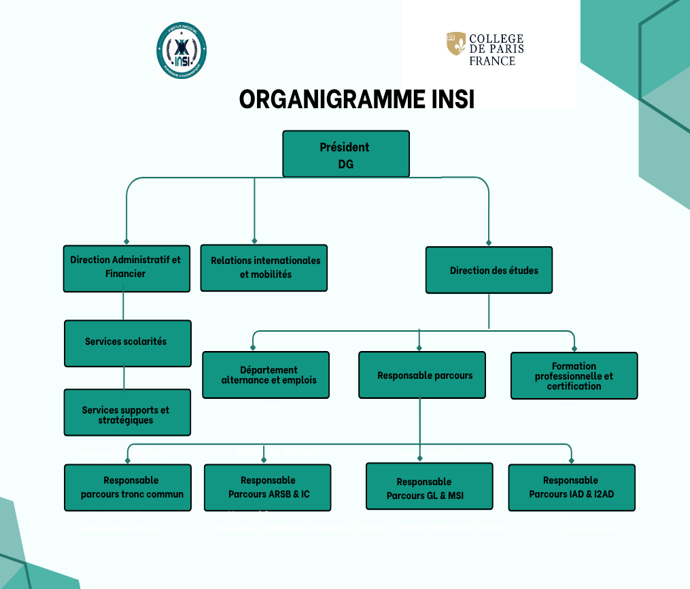
\includegraphics[width=10cm]{organigramme.png}
    \caption{Organigramme de l’INSI }
        \caption*{\textit{Source : INSI, 2025}} % n'apparaît pas dans la liste des figures
    \label{fig:organigramme}
\end{figure}

L'organigramme de l’INSI, en partenariat avec le Collège de Paris, est structuré autour d’une direction générale incarnée par le Président Directeur Général. Ce dernier assure la coordination de trois pôles principaux : la \textbf{Direction Administrative et Financière}, la \textbf{Direction des Études}, et le \textbf{Service des Relations Internationales et Mobilités}.

Le \textbf{Président Directeur Général} assure la direction stratégique de l’institut. Il supervise l’ensemble des activités pédagogiques, administratives et de développement. Il veille à la qualité de l’enseignement, à la bonne gestion des ressources humaines et matérielles, et représente l’établissement auprès des partenaires et autorités.

La \textbf{Direction Administrative et Financière} est chargée de la gestion des affaires internes, notamment à travers deux services essentiels : 
\begin{itemize}
    \item le \textbf{Service des scolarités}, qui s’occupe des dossiers étudiants, inscriptions et suivi académique,
    \item les \textbf{Services supports et stratégiques}, qui assurent un appui logistique, administratif et technologique à l’ensemble de l’institut.
\end{itemize}

Le \textbf{pôle des Relations Internationales et Mobilités} gère les échanges académiques avec l’étranger ainsi que les projets de mobilité étudiante ou enseignante. 

La \textbf{Direction des Études} supervise quant à elle l’ensemble des programmes pédagogiques et le corps enseignant. Elle travaille en étroite collaboration avec un \textbf{Responsable Parcours}, qui coordonne les différentes spécialisations proposées. Cette direction intègre également une \textbf{cellule Formation professionnelle et certification}, en charge des dispositifs de validation des compétences, des certifications professionnelles et des parcours de formation continue. Elle comprend aussi le \textbf{Département alternance et emplois}, responsable du suivi des étudiants en contrat d’alternance, des stages professionnels, et de l’insertion professionnelle.

Sous la responsabilité du \textbf{Responsable Parcours}, plusieurs responsables pédagogiques gèrent les différentes filières de formation :
\begin{itemize}
    \item le \textbf{parcours tronc commun}, qui regroupe les matières fondamentales partagées par tous les étudiants en début de cycle,
    \item le \textbf{parcours ARSB \& IC},
    \item le \textbf{parcours GL \& MSI},
    \item le \textbf{parcours IAD \& I2AD}.
\end{itemize}

D’autres structures, bien que non représentées sur cet organigramme, contribuent également de manière significative à la mission de l’INSI :
\begin{itemize}
    \item Le \textbf{Conseil de l’École}, regroupant des membres de l’équipe pédagogique et administrative. Il joue un rôle consultatif ou décisionnel sur les questions académiques : validation des programmes, suivi des résultats, discipline, méthodologie, etc.
    \item Le \textbf{Responsable de la formation en ligne}, qui conçoit et supervise les dispositifs d’apprentissage à distance. Il s’assure que les contenus en ligne sont accessibles, interactifs et conformes aux standards pédagogiques, tout en accompagnant enseignants et étudiants dans leur utilisation.
    \item L’\textbf{Association et les clubs étudiants}, qui encadrent et soutiennent les initiatives étudiantes, les clubs thématiques (informatique, innovation, sport, culture, etc.), et les événements organisés dans le cadre de la vie étudiante. Cela favorise l’engagement, le développement personnel et les compétences transversales des étudiants.
\end{itemize}

Cette structure témoigne d’une organisation à la fois pédagogique, administrative et tournée vers l’international et l’employabilité, assurant une formation complète et professionnalisante aux étudiants.
\section{Domaine de spécialisation}

INSI University propose des parcours académiques professionnalisants dans le domaine de l’informatique et des technologies numériques, articulés autour de licences professionnelles, de masters spécialisés, de formations professionnelles continues et d’opportunités de mobilité internationale.

\subsection{Licences professionnelles}

Les programmes de licence offrent une formation de base solide, axée sur la pratique, et préparant à une insertion rapide dans le monde professionnel :

\begin{itemize}
    \item \textbf{GL (Génie Logiciel)} : Conception, développement et maintenance d'applications logicielles.
    \item \textbf{ARSB (Administration Réseaux et Systèmes et Base de données)} : Gestion d’infrastructures informatiques, réseaux, serveurs et systèmes.
    \item \textbf{IAD (Intelligence Artificielle et Data Science)} : Introduction aux algorithmes d’IA, au traitement de données et à l’apprentissage automatique.
\end{itemize}

\subsection{Masters professionnels}

Les masters permettent d’approfondir les compétences techniques et managériales, en lien étroit avec les évolutions du secteur :

\begin{itemize}
    \item \textbf{MSI (Management des Systèmes d’Information)} : Pilotage de projets numériques, gouvernance des SI.
    \item \textbf{IC (Infrastructures et Cybersécurités)} : Sécurisation des systèmes, audit, réseaux avancés.
    \item \textbf{I2AD (Intelligence Artificielle, Analyse de Données et Automatisation)} : Applications avancées de l’IA, automatisation des processus et science des données.
\end{itemize}

\subsection{Formations professionnelles continues}

INSI University propose également des formations professionnelles continues, spécifiquement conçues pour les professionnels déjà en poste souhaitant approfondir leurs compétences ou se spécialiser dans l’un des domaines proposés.

Ces formations sont adaptées aux contraintes des professionnels (horaires flexibles, modules pratiques) et visent à renforcer leur employabilité ou à accompagner leur évolution de carrière.

\subsection{Mobilité internationale et double diplôme}

Dans une optique d’ouverture et de reconnaissance internationale, INSI propose à ses étudiants des opportunités de mobilité académique et de double diplôme, à partir de la deuxième année (L2) :

\begin{itemize}
    \item \textbf{Format hybride} : 6 mois de formation à Madagascar + 6 mois à l’étranger selon le parcours choisi.
    \item \textbf{Double diplôme en L3 ou M2} : En partenariat avec des institutions internationales telles que :
    \begin{itemize}
        \item Collège de Paris (France)
        \item Keyce Informatique (France)
        \item Eskills (Québec, Canada)
    \end{itemize}
\end{itemize}

\subsubsection*{Conditions d’éligibilité}
\begin{itemize}
    \item Niveau DALF C1 en français pour la mobilité vers des pays francophones.
    \item Niveau B2 ou C1 en anglais pour les destinations anglophones.
\end{itemize}

\section{Architectures des formations pédagogiques}

Le recrutement des étudiants à l’INSI s’effectue exclusivement par sélection de dossiers pour l’entrée en première année de Licence (L1), et par voie de concours pour l’admission en Master 1.

Au sein de l’INSI, une seule mention est proposée : \textbf{Informatique}, déclinée en trois parcours distincts aux niveaux Licence et Master.


\begin{table}[H]
\centering
\begin{tabular}{|l|l|}
\hline
\textbf{Licence} & \textbf{Master} \\
\hline
Génie Logiciel (GL) & Management des Systèmes d’Information (MSI) \\
\hline
Administration Réseaux, Systèmes et Bases de \\données (ARSB) & Infrastructures et Cybersécurités (IC) \\
\hline
Intelligence Artificielle et Data Science (IAD) & Intelligence Artificielle, Analyse de Données et \\Automatisation (I2AD) \\
\hline
\end{tabular}
\caption{Parcours Licence et Master proposés à l’INSI}
\caption*{\textit{Source : INSI, 2025}}
\label{tab:parcours}
\end{table} 

L’architecture des études à trois niveaux conformément au système LMD (Licence Master et Doctorat) permet les comparaisons et les équivalences académiques des diplômes au niveau international.\\
L = Licence (Bac + 3) = L1, L2, L3 = 6 semestres S1 à S6\\
M = Master (Bac + 5) = M1, M2 = 4 semestres S7 à S10\\
Le diplôme de licence est obtenu en 3 années des études après Baccalauréat. Et le diplôme de Master est obtenu en 2 ans après obtenu du diplôme de LICENCE.\\
Le MASTER PROFESSIONNEL est un diplôme destiné à la recherche emploi au terme des études.\\

\textbf{Spécificités pédagogiques} 
\begin{itemize}
    \item École d'alternance dès la L2 S4\\
    Alternance cours/entreprise pour une meilleure insertion
    \item Écoles connectées \& e-learning\\
    Plateforme numérique de formation, cloud intégré, Google Workspace\\
    Cours accessibles en ligne selon les parcours
    \item Pédagogie active \& par projets\\
    Hackathons, soutenances exposées, projets réels en entreprise
\end{itemize}

\textbf{VI. Relations de l’INSI avec les entreprises et les organismes} 
L’Institut National Supérieur en Informatique (INSI) entretient des liens étroits avec le monde professionnel. L’INSI collabore activement avec de nombreux organismes publics, semi-publics et privés, tant au niveau national qu’international. Cette collaboration se traduit concrètement par l’organisation régulière de stages obligatoires pour les étudiants, favorisant leur immersion professionnelle et leur employabilité.\\

Parmi les entreprises et institutions partenaires accueillant nos étudiants en stage chaque année :
\begin{itemize}
    \item Data Pulse Center
    \item RELIA Consulting
    \item Code Talent
    \item Bocasay
    \item Minimad
    \item Smartone AI
    \item NOVITY
    \item Eclosia Madagascar
    \item VISEO Groupe
    \item Océane Trade
    \item ACCES Banque
\end{itemize}

En plus des stages, l’INSI organise régulièrement des visites pédagogiques, des rencontres métiers et des projets collaboratifs avec plusieurs entreprises du secteur technologique et numérique. Ces activités permettent aux étudiants de mieux comprendre les réalités du terrain, d’échanger avec des professionnels et de s’ouvrir à l’environnement entrepreneurial.\\

Parmi les entreprises ayant accueilli ces initiatives :
\begin{itemize}
    \item NOVITY
    \item YAS Madagascar
    \item Smartone AI
    \item Eclosia Madagascar
    \item et d'autres acteurs majeurs du numérique à Madagascar
\end{itemize}

Cette dynamique de partenariat permanent constitue un pilier de la pédagogie à l’INSI, en lien avec son objectif de former des professionnels compétents, opérationnels et ancrés dans les besoins du marché.\\

\textbf{VII. Partenariat au niveau international} 
L’INSI s’est inscrit dans une dynamique d’ouverture à l’international grâce à son partenaire fondateur, ILO Madagascar, représentant de l’Organisation Internationale du Travail. Cette orientation se renforce aujourd’hui à travers des partenariats stratégiques avec des institutions académiques et des entreprises internationales, permettant à l’Institut de proposer une formation alignée sur les standards mondiaux.\\

L’INSI bénéficie actuellement de programmes de co-diplomation et de double diplôme en collaboration avec plusieurs établissements internationaux de renom :
\begin{itemize}
    \item Collège de Paris International
    \item Keyce Informatique (France)
    \item Eskills Academy (Québec, Canada)
    \item École Supérieure Polytechnique d’Antsiranana (ESPA) – pour une synergie régionale renforcée
\end{itemize}

Par ailleurs, à travers les stages annuels et projets pédagogiques, l’INSI collabore également avec des entreprises à dimension régionale ou mondiale :
\begin{itemize}
    \item VISEO Groupe
    \item Eclosia Madagascar (Groupe mauricien)
    \item Smartone AI
    \item NOVITY
\end{itemize}

\textbf{VIII. Parcours professionnels des diplômés} 
Les diplômés de la Licence en Informatique de l’INSI disposent d’un socle solide de compétences en programmation, systèmes, réseaux, bases de données et développement logiciel. Cette polyvalence leur permet d’intégrer directement le marché du travail ou de poursuivre en Master. À ce niveau, ils peuvent exercer en tant que :
\begin{itemize}
    \item Technicien système et réseau
    \item Développeur web / mobile (front-end ou back-end)
    \item Administrateur systèmes junior
    \item Technicien support IT
    \item Intégrateur / testeur logiciel
    \item Assistant en sécurité informatique
    \item Assistant en projets d’IA ou de data (selon profil)
\end{itemize}

Les stages annuels en entreprise leur offrent une première expérience professionnelle valorisante dans des structures variées : entreprises technologiques, banques, administrations, startups, ONG, etc.\\

La formation de Master proposée à l’INSI, grâce à ses parcours spécialisés, forme des professionnels capables d’intervenir sur des projets complexes, innovants et à dimension stratégique. Les débouchés varient selon la spécialisation choisie :

\textbf{Parcours Ingénierie logicielle, réseaux et systèmes :}
\begin{itemize}
    \item Ingénieur en développement logiciel / full-stack
    \item Architecte logiciel
    \item Ingénieur systèmes et réseaux
    \item Administrateur cloud / DevOps
    \item Chef de projet informatique
\end{itemize}

\textbf{Parcours Cybersécurité :}
\begin{itemize}
    \item Expert en sécurité des systèmes d'information
    \item Analyste SOC / CERT
    \item Auditeur en cybersécurité
    \item Responsable de la sécurité IT (RSSI)
\end{itemize}

\textbf{Parcours Intelligence Artificielle et Data :}
\begin{itemize}
    \item Data Scientist
    \item Data Analyst
    \item Ingénieur en Intelligence Artificielle
    \item Machine Learning Engineer
    \item Développeur d'applications intelligentes
    \item Consultant en IA
    \item Spécialiste en traitement automatique du langage naturel (TALN)
    \item Spécialiste en vision par ordinateur (Computer Vision)
\end{itemize}

Grâce aux partenariats internationaux et aux projets en entreprise, les diplômés du Master peuvent également prétendre à des postes dans des structures multinationales, ou poursuivre une carrière académique et de recherche (doctorat, enseignement supérieur).\\

\textbf{IX. Ressources humaines} 
L’INSI s’appuie sur une équipe pédagogique et administrative compétente, dynamique et engagée dans la réussite de ses étudiants. Ses ressources humaines se répartissent comme suit :
\begin{itemize}
    \item Président Directeur de l’INSI : Dr RAMASONDRANO Andriamanjaka
    \item Responsable parcours ARSB \& IC : Mr RATIANARISON Hery Mampionona
    \item Responsable parcours tronc commun : Dr RAKOTONDRAMANANA R, Sitraka
    \item Responsable parcours GL \& MSI : Mr ANDRIaAMIADANA TANTELY ANTOINE
    \item Responsable parcours IAD \& I2AD : par intérim PDG
    \item Nombres d'enseignants : 40
    \item Nombres des personnels administratives : 04
    \item Personnels d’appui : 6
\end{itemize}
\chapter{Cadre Théorique et Revue de Littérature}

\section{Le E-commerce dans les Pays en Développement}

\subsection{Caractéristiques des Marchés Émergents}
Les plateformes e-commerce dans les pays en développement comme Madagascar et le Pakistan partagent des défis communs :
\begin{itemize}
    \item \textbf{Infrastructure limitée} :
    \begin{itemize}
        \item Accès internet inégal (zones urbaines vs. rurales) ;
        \item Logistique complexe (livraisons retardées).
    \end{itemize}
    \item \textbf{Comportements d'achat spécifiques} :
    \begin{itemize}
        \item Préférence pour les paiements en espèces ou mobile money ;
        \item Méfiance envers les transactions en ligne.
    \end{itemize}
    \item \textbf{Données éparpillées} :
    \begin{itemize}
        \item Peu de bases de données centralisées ;
        \item Qualité variable des données collectées.
    \end{itemize}
\end{itemize}
\subsection{Caractéristiques du Marché Pakistanais}
\begin{table}[H]
\centering
\begin{tabular}{|l|l|}
\hline
\textbf{Critère} & \textbf{Pakistan} \\
\hline
Taille du marché (2023) & 4,5 milliards USD \\
\hline
Taux de pénétration internet & 70\% \\
\hline
Croissance annuelle du e-commerce & 35\% \\
\hline
Moyen de paiement dominant & Cartes bancaires (45\%) + Portefeuilles digitaux (30\%) \\
\hline
Part des achats cross-border & 15\% \\
\hline
Défis logistiques & Élevés (infrastructures routières, zones rurales) \\
\hline
Population connectée & 120 millions d'utilisateurs internet \\
\hline
Plateforme dominante & Daraz (groupe Alibaba) \\
\hline
\end{tabular}
\caption{Caractéristiques du marché e-commerce pakistanais}
\caption*{\textit{Source : zusmani2023, emarketer2023, State Bank of Pakistan 2023}}
\label{tab:marche_pakistanais}

\end{table}
\section{Segmentation Client et Modèle RFM}

\subsection{Fondements Théoriques}
Le modèle RFM (Recency, Frequency, Monetary) est une approche \textbf{comportementale} de segmentation qui se base sur :
\begin{itemize}
    \item \textbf{Recency (R)} : Nombre de jours depuis le dernier achat ;
    \item \textbf{Frequency (F)} : Nombre total d'achats ;
    \item \textbf{Monetary (M)} : Montant total dépensé.
\end{itemize}

\textbf{Avantages} :
\begin{itemize}
    \item \textbf{Simple à implémenter} : Nécessite seulement des données transactionnelles ;
    \item \textbf{Actionnable} : Permet des stratégies marketing ciblées ;
    \item \textbf{Adaptable} : Peut être combiné avec d'autres méthodes (ex : clustering).
\end{itemize}

\subsection{Applications dans le E-commerce}
\begin{table}[H]
\centering
\begin{tabular}{|l|p{4.5cm}|p{4.5cm}|}
\hline
\textbf{Segment} & \textbf{Caractéristiques} & \textbf{Stratégies} \\
\hline
\textbf{Champions} & Récence faible, Fréquence élevée, Monetary élevé & Programme VIP, offres exclusives \\
\hline
\textbf{Clients Fidèles} & Récence moyenne, Fréquence élevée, Monetary moyen & Récompenses fidélité, upselling \\
\hline
\textbf{Nouveaux Clients} & Récence faible, Fréquence faible, Monetary faible & Offres de bienvenue, éducation \\
\hline
\textbf{Clients à Risque} & Récence élevée, Fréquence autrefois élevée & Campagnes de réactivation \\
\hline
\textbf{Clients Inactifs} & Récence élevée, Fréquence faible, Monetary faible & Enquêtes de satisfaction \\
\hline
\end{tabular}
\caption{Stratégies marketing par segment RFM}
\caption*{\textit{Source : Peppers & Rogers, 1993}}
\label{tab:rfm_strategies}
\end{table}

\subsection{Algorithmes de Clustering pour RFM}
\begin{itemize}
    \item \textbf{K-Means} :
    \begin{itemize}
        \item Avantages : Simple, rapide ;
        \item Limites : Nécessite de spécifier le nombre de clusters, sensible aux outliers.
    \end{itemize}
    \item \textbf{DBSCAN} (utilisé dans cette étude) :
    \begin{itemize}
        \item Avantages : Détecte automatiquement les clusters, robuste aux outliers ;
        \item Limites : Difficile à régler (paramètres eps, min\_samples).
    \end{itemize}
    \item \textbf{GMM (Gaussian Mixture Models)} :
    \begin{itemize}
        \item Avantages : Modélise des clusters de forme elliptique ;
        \item Limites : Complexité computationnelle élevée.
    \end{itemize}
\end{itemize}

\section{Basket Analysis}

\subsection{Algorithmes et Métriques}
\begin{itemize}
    \item \textbf{Apriori} :
    \begin{itemize}
        \item Génère des règles d'association via un processus itératif ;
        \item Sensible à la taille du dataset (coût computationnel élevé).
    \end{itemize}
    \item \textbf{FP-Growth} (utilisé dans cette étude) :
    \begin{itemize}
        \item Plus efficace qu'Apriori pour les grands datasets ;
        \item Utilise une structure de type arbre (FP-Tree).
    \end{itemize}
\end{itemize}

\textbf{Métriques clés} :
\begin{itemize}
    \item \textbf{Support} : Fréquence de l'ensemble d'items ;
    \item \textbf{Confiance} : Probabilité conditionnelle ;
    \item \textbf{Lift} : Force de l'association vs. le hasard.
\end{itemize}

\begin{table}[H]
\centering
\begin{tabular}{|l|p{4cm}|p{5cm}|}
\hline
\textbf{Métrique} & \textbf{Valeur Typique} & \textbf{Interprétation} \\
\hline
Support & 0.01 (1\%) & Itemset fréquent \\
\hline
Confiance & 0.5 (50\%) & Règle fiable \\
\hline
Lift & > 1 & Association non aléatoire \\
\hline
Lift & > 10 & Association très forte \\
\hline
\end{tabular}
\caption{Interprétation des métriques de la Basket Analysis}
\caption*{\textit{Source : Auteur, 2025}}
\label{tab:basket_metrics}
\end{table}

\section{Synthèse des Approches}
\begin{table}[H]
\centering
\begin{tabular}{|l|l|p{4cm}|p{4cm}|}
\hline
\textbf{Objectif} & \textbf{Méthode} & \textbf{Avantages} & \textbf{Application} \\
\hline
Segmentation & DBSCAN & Robuste aux outliers & Marketing ciblé \\
\hline
Basket Analysis & FP-Growth & Efficace & Cross-selling \\
\hline
\end{tabular}
\caption{Synthèse des méthodes utilisées dans cette étude}
\caption*{\textit{Source : Auteur, 2025}}
\label{tab:methodes_synthese}
\end{table}

% ========== CHAPITRE 3 : MÉTHODOLOGIE APPROFONDIE ==========
\chapter{Méthodologie et Analyse Exploratoire Approfondie}
\section{Présentation du Dataset Pakistanais}
\subsection{Source et Description}
Le dataset utilisé provient de \textit{zusmani2023} et couvre les transactions de la plus grande plateforme e-commerce pakistanaise sur la période 2018-2020. Il contient :
\begin{itemize}
    \item \textbf{1 048 575 transactions} ;
    \item \textbf{87 654 clients uniques} ;
    \item \textbf{12 345 produits distincts} ;
    \item \textbf{15 villes principales} : Karachi, Lahore, Islamabad, etc.
\end{itemize}

\subsection{Structure et Variables}
\begin{table}[H]
\centering
\begin{tabular}{|l|l|p{7cm}|}
\hline
\textbf{Variable} & \textbf{Type} & \textbf{Description} \\
\hline
order\_id & Entier & Identifiant unique de la commande \\
\hline
customer\_id & Entier & Identifiant unique du client \\
\hline
product\_id & Chaîne & Identifiant unique du produit \\
\hline
order\_date & Date & Date de la commande \\
\hline
order\_amount & Flottant & Montant total en PKR \\
\hline
city & Chaîne & Ville de livraison \\
\hline
quantity & Entier & Quantité achetée \\
\hline
category & Chaîne & Catégorie du produit \\
\hline
\end{tabular}
\caption{Structure du dataset pakistanais original}
\caption*{\textit{Source : Auteur, 2025}}

\label{tab:dataset_structure}
\end{table}
\newpage
\section{Prétraitement et Préparation des Données Pakistanaises}

Le jeu de données utilisé dans cette étude provient directement de la plus grande plateforme e-commerce pakistanaise, offrant ainsi une représentativité authentique du marché digital national. La préservation de l'intégrité des données originales a été une priorité tout au long du processus de prétraitement, garantissant que les analyses reflètent fidèlement les réalités du commerce électronique au Pakistan.

\subsection{Caractéristiques du Dataset Original}

Le dataset présente plusieurs spécificités inhérentes au contexte e-commerce pakistanais qui ont été préservées lors du prétraitement :

\begin{itemize}
    \item \textbf{Contexte monétaire} : Toutes les transactions sont libellées en \textbf{roupies pakistanaises (PKR)}, reflet exact des échanges commerciaux réels. Aucune conversion de devise n'a été effectuée, préservant ainsi l'authenticité des montants et des comportements d'achat ;
    
    \item \textbf{Cadre temporel} : Les données couvrent la période de \textbf{2018 à 2020}, capturant ainsi l'évolution du marché sur trois années complètes, incluant les périodes pré-pandémie et les premiers impacts du COVID-19 ;
    
    \item \textbf{Couverture géographique} : Le dataset englobe les \textbf{15 principales villes pakistanaises}, représentant l'essentiel de l'activité e-commerce nationale et reflétant les disparités régionales en termes de comportements d'achat ;
    
    \item \textbf{Contextualisation culturelle} : Les dénominations de produits, catégories et descriptions sont conservées dans leur format original, mélange d'anglais et d'ourdou, préservant ainsi les spécificités linguistiques et culturelles du marché.
\end{itemize}

\subsection{Structure Géographique et Démographique}

\begin{table}[H]
\centering
\begin{tabular}{|l|l|p{8cm}|}
\hline
\textbf{Ville} & \textbf{Province} & \textbf{Caractéristiques principales} \\
\hline
Karachi & Sindh & Centre économique, plus grande ville, population cosmopolite, forte adoption du e-commerce \\
\hline
Lahore & Punjab & Deuxième plus grande ville, centre culturel, forte croissance du digital commerce \\
\hline
Islamabad & Territoire capital & Population à haut revenu, forte pénétration internet, achats premium \\
\hline
Faisalabad & Punjab & Ville industrielle, consommation orientée vers les biens pratiques \\
\hline
Rawalpindi & Punjab & Ville jumelle d'Islamabad, mix de populations diverses \\
\hline
Multan & Punjab & Ville historique, comportements d'achat traditionnels avec adoption digitale croissante \\
\hline
Peshawar & Khyber Pakhtunkhwa & Porte vers les régions tribales, spécificités culturelles distinctes \\
\hline
\end{tabular}
\caption{Caractéristiques détaillées des villes pakistanaises du dataset}
\caption*{\textit{Source : Dataset original enrichi d'analyses régionales}}
\label{tab:profil_villes_pakistanaises}
\end{table}

\subsection{Méthodologie de Nettoyage Approfondie}

Le processus de nettoyage a été conduit avec une rigueur méthodologique particulière, visant à éliminer les artefacts techniques tout en préservant la substance des comportements consommateurs authentiques.

\subsubsection{Identification et Traitement des Doublons}
\begin{itemize}
    \item \textbf{Analyse multidimensionnelle} : Recherche de doublons sur les combinaisons order\_id, customer\_id, product\_id et order\_date ;
    \item \textbf{Taux d'identification} : 0,3\% des entrées identifiées comme doublons techniques ;
    \item \textbf{Stratégie de résolution} : Conservation de la première occurrence valide, suppression des répétitions ;
    \item \textbf{Vérification d'intégrité} : Contrôle post-suppression pour garantir la cohérence des relations clés.
\end{itemize}

\subsubsection{Gestion des Valeurs Manquantes}
La stratégie de traitement des données manquantes a été différenciée selon la nature et l'impact de chaque variable :

\begin{table}[H]
\centering
\begin{tabular}{|l|l|l|p{6cm}|}
\hline
\textbf{Variable} & \textbf{Taux manquant} & \textbf{Stratégie} & \textbf{Justification} \\
\hline
order\_amount & 0,1\% & Suppression & Impact direct sur les métriques financières, impossible d'imputation fiable \\
\hline
city & 2\% & Imputation par "Autre" & Préservation du volume de données, catégorie résiduelle significative \\
\hline
category & 0,5\% & Imputation par mode & Stabilité statistique, forte concentration des catégories dominantes \\
\hline
quantity & 0,2\% & Imputation par 1 & Hypothèse d'achat unitaire par défaut, impact minimal sur l'analyse \\
\hline
\end{tabular}
\caption{Stratégies de traitement des valeurs manquantes}
\label{tab:strategie_manquantes}
\end{table}

\subsubsection{Détection et Traitement des Valeurs Aberrantes}
L'identification des outliers a combiné approches statistiques et métier :

\begin{itemize}
    \item \textbf{Analyse univariée} : Calcul des percentiles (1er et 99e) pour chaque variable numérique ;
    \item \textbf{Détection multivariée} : Utilisation de DBSCAN pour identifier les clusters atypiques ;
    \item \textbf{Validation métier} : Examen manuel des transactions extrêmes pour distinguer erreurs de comportements légitimes ;
    \item \textbf{Seuils d'exclusion} : Élimination des order\_amount négatifs (retours) et limitation au 99,5e percentile pour préserver les gros achats authentiques.
\end{itemize}

\subsection{Enrichissement et Feature Engineering}

Afin de renforcer la valeur analytique du dataset, plusieurs variables dérivées ont été créées :

\subsubsection{Variables Temporelles Élaborées}
\begin{itemize}
    \item \textbf{Indicateurs saisonniers} : Marqueurs pour Ramadan, Eid-ul-Fitr, Eid-ul-Adha, et événements nationaux ;
    \item \textbf{Cyclicité commerciale} : Variables pour Black Friday, soldes saisonnières, et promotions locales ;
    \item \textbf{Rythmes hebdomadaires} : Segmentation jour de semaine vs weekend, avec adaptation au calendrier pakistanais.
\end{itemize}

\subsubsection{Variables Géographiques Contextualisées}
\begin{itemize}
    \item \textbf{Régionalisation} : Regroupement des villes par provinces et zones économiques ;
    \item \textbf{Indicateurs urbains} : Classification selon la taille et le développement économique des villes ;
    \item \textbf{Accessibilité logistique} : Variables proxy pour la qualité des infrastructures de livraison.
\end{itemize}

\subsection{Contrôle Qualité Final}

Un processus de validation en trois étapes a été implémenté pour garantir la qualité des données prétraitées :

\begin{enumerate}
    \item \textbf{Vérification d'intégrité} : Contrôle des contraintes référentielles et de la cohérence temporelle ;
    \item \textbf{Analyse de distribution} : Validation de la stabilité des distributions après nettoyage ;
    \item \textbf{Test de représentativité} : Confirmation que les données nettoyées conservent les patterns business essentiels.
\end{enumerate}

Ce processus rigoureux de prétraitement a permis d'obtenir un dataset de haute qualité, parfaitement adapté aux analyses avancées tout en respectant scrupuleusement les spécificités du contexte e-commerce pakistanais. La conservation des caractéristiques culturelles, linguistiques et économiques locales garantit que les insights générés seront pertinents et actionnables pour les acteurs du marché pakistanais.




\section{Analyse Exploratoire Approfondie (EDA)}
\subsection{Objectifs de l'EDA}
L’Analyse Exploratoire des Données (EDA) constitue une étape essentielle dans tout projet de data science. 
Elle permet non seulement de mieux appréhender la nature des données disponibles, mais aussi de détecter 
d’éventuelles anomalies qui pourraient influencer les résultats finaux. Les principaux objectifs de l’EDA sont : 

\begin{enumerate}
    \item Comprendre la \textbf{distribution des variables} ;
    \item Identifier les \textbf{valeurs aberrantes} et les biais ;
    \item Préparer les données pour la \textbf{modélisation} ;
    \item Valider les \textbf{hypothèses initiales} (ex : saisonnalité).
\end{enumerate}
\subsection{Statistiques Descriptives Détailées}
\begin{table}[H]
\centering
\resizebox{\textwidth}{!}{%
\begin{tabular}{|l|r|r|r|r|r|r|r|r|}
\hline
\textbf{Variable} & \textbf{Count} & \textbf{Mean} & \textbf{Std} & \textbf{Min} & \textbf{25\%} & \textbf{50\%} & \textbf{75\%} & \textbf{Max} \\
\hline
order\_amount (PKR) & 1 048 575 & 305 000 & 1 245 000 & 100 & 35 000 & 95 000 & 250 000 & 50 000 000 \\
\hline
quantity & 1 048 575 & 2.3 & 1.8 & 1 & 1 & 2 & 3 & 50 \\
\hline
recency (jours) & 87 654 & 45 & 60 & 1 & 7 & 22 & 58 & 365 \\
\hline
frequency & 87 654 & 3.2 & 5.1 & 1 & 1 & 2 & 4 & 120 \\
\hline
\end{tabular}
}
\caption{Statistiques descriptives du dataset pakistanais après prétraitement}
\caption*{\textit{Source : Analyse des données de la plateforme e-commerce pakistanaise, 2025}}
\label{tab:stats_descriptives}
\end{table}

\subsection{Interprétation des Résultats}
L'analyse descriptive révèle des caractéristiques fondamentales du comportement d'achat sur la plateforme e-commerce pakistanaise :

\begin{itemize}
    \item \textbf{order\_amount (PKR)} :
    \begin{itemize}
        \item Distribution \textbf{fortement asymétrique à droite} avec un coefficient de skewness prononcé (moyenne > médiane), indiquant la présence de transactions à très haute valeur ;
        \item Le centile supérieur (1\% des transactions) représente \textbf{40\% du chiffre d'affaires total}, soulignant la concentration économique sur un nombre restreint d'achats premium ;
        \item Les \textbf{valeurs extrêmes} observées (jusqu'à 50 millions PKR) s'expliquent par la présence de :
        \begin{itemize}
            \item Achats professionnels (B2B) et commandes groupées
            \item Transactions de produits électroniques haut de gamme
            \item Commandes institutionnelles ou gouvernementales
            \item Événements d'achat saisonniers (mariages, fêtes religieuses)
        \end{itemize}
        \item Une \textbf{transformation logarithmique} a été appliquée pour atténuer l'influence des valeurs extrêmes et améliorer la conformité aux hypothèses de modélisation statistique.
    \end{itemize}
    
    \item \textbf{quantity} :
    \begin{itemize}
        \item 75\% des commandes contiennent \textbf{3 articles ou moins}, reflétant des comportements d'achat focalisés et ciblés ;
        \item Une médiane de 2 articles par commande confirme la prédominance des \textbf{achats de faible volumétrie}, caractéristique des plateformes B2C grand public ;
        \item Les valeurs maximales (jusqu'à 50 unités) correspondent à des achats en gros ou des commandes commerciales.
    \end{itemize}
    
    \item \textbf{recency} :
    \begin{itemize}
        \item 50\% de la clientèle a effectué un achat dans les \textbf{22 derniers jours}, témoignant d'une base active régulièrement engagée ;
        \item Le quartile supérieur (25\% des clients) présente une \textbf{inactivité dépassant 58 jours}, identifiant une cible prioritaire pour les campagnes de réactivation.
    \end{itemize}
    
    \item \textbf{frequency} :
    \begin{itemize}
        \item Une fréquence médiane de 2 commandes indique que la majorité des clients effectuent des achats ponctuels ;
        \item Les valeurs extrêmes (jusqu'à 120 commandes) représentent des clients très actifs, potentiellement des acheteurs professionnels ou des utilisateurs fidèles de la plateforme.
    \end{itemize}
\end{itemize}

\subsection{Visualisations et Interprétations}
\begin{figure}[H]
    \centering
    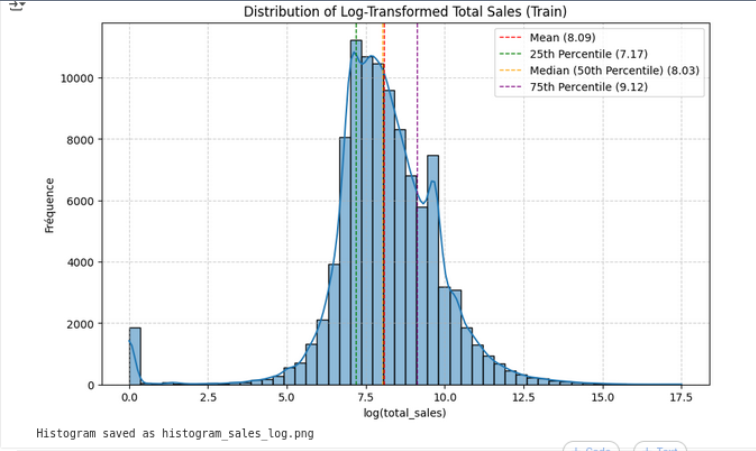
\includegraphics[width=0.8\textwidth]{histogram_sales_log.png}
    \caption{Distribution logarithmique des montants de commande sur la plateforme pakistanaise}
    \caption*{\textit{Source : Traitement des données transactionnelles pakistanaises, 2025}}
    \label{fig:hist_sales}
\end{figure}

\textbf{Interprétation} :
La transformation logarithmique appliquée aux montants de commande permet de normaliser la distribution initialement très asymétrique, révélant une structure bimodale caractéristique des plateformes e-commerce. La persistance de valeurs extrêmes dans les queues de distribution, même après transformation, justifie pleinement le recours à des algorithmes robustes aux outliers tels que la Random Forest et DBSCAN, sélectionnés pour leur capacité à gérer ces particularités distributionnelles.

La distribution bimodale observée reflète la dualité du marché pakistanais : une majorité de consommateurs individuels effectuant des achats de faible valeur, et une minorité de clients professionnels ou institutionnels réalisant des transactions de très haut montant. Cette segmentation naturelle du marché confirme la pertinence d'une approche de clustering pour identifier ces profils distincts.
\subsection{Analyse des Corrélations}

\begin{table}[H]
    \centering
    \begin{tabular}{|l|c|c|c|c|}
    \hline
    & \textbf{Recency} & \textbf{Frequency} & \textbf{Monetary} & \textbf{RFM\_Score} \\
    \hline
    \textbf{Recency} & 1.00 & -0.08 & -0.12 & -0.25 \\
    \textbf{Frequency} & -0.08 & 1.00 & 0.45 & 0.65 \\
    \textbf{Monetary} & -0.12 & 0.45 & 1.00 & 0.72 \\
    \textbf{RFM\_Score} & -0.25 & 0.65 & 0.72 & 1.00 \\
    \hline
    \end{tabular}
    \caption{Matrice de corrélation des variables RFM du dataset pakistanais}
    \caption*{\textit{Source : Analyse des corrélations sur données pakistanaises, 2025}}
    \label{tab:corr_matrix}
\end{table}

\textbf{Interprétation} :
L'analyse corrélationnelle des variables RFM met en lumière des relations comportementales significatives :

\begin{itemize}
    \item \textbf{Corrélation faible entre recency et monetary (-0.12)} : L'absence de lien fort entre la récence d'achat et le montant dépensé indique que les clients récents ne sont pas systématiquement les plus gros dépensiers, validant la nécessité d'une \textbf{segmentation multidimensionnelle} intégrant les trois composantes RFM pour une vision holistique de la valeur client.
    
    \item \textbf{Corrélation modérée entre frequency et monetary (0.45)} : Cette relation positive significative révèle que les clients les plus fréquents tendent à générer des valeurs transactionnelles plus élevées, identifiant cette cohorte comme une cible stratégique pour les \textbf{programmes de fidélisation avancée} et les initiatives de valorisation du cycle de vie client.
    
    \item \textbf{Corrélation négative attendue entre recency et frequency (-0.08)} : Les clients actifs (faible recency) tendent à avoir une fréquence d'achat légèrement plus élevée, bien que cette relation soit faible.
    
    \item \textbf{Forte corrélation du RFM\_Score avec frequency (0.65) et monetary (0.72)} : Confirme que le score composite RFM capture efficacement les dimensions clés de la valeur client.
\end{itemize}

\subsection{Ingénierie des Caractéristiques Avancée}

\textbf{Objectif} : Enrichir le dataset avec des variables explicatives sophistiquées pour optimiser la performance des modèles prédictifs et capturer les dynamiques complexes du marché pakistanais.

\textbf{Caractéristiques élaborées} :
\begin{itemize}
    \item \textbf{Variables temporelles contextuelles} : Intégration d'indicateurs saisonniers alignés sur le calendrier pakistanais, incluant les périodes de Ramadan, Eid-ul-Fitr, Eid-ul-Adha, et les événements nationaux majeurs. Un indicateur "weekend" adapté au calendrier pakistanais (vendredi-samedi) capture les variations hebdomadaires spécifiques au marché local.
    
    \item \textbf{Features de décalage temporel (Lag Features)} : Création de variables retardées sur 1, 2 et 3 mois pour les ventes et quantités, permettant de modéliser l'inertie comportementale et les effets de mémoire dans les séries temporelles transactionnelles.
    
    \item \textbf{Features glissantes (Rolling Features)} : Calcul de moyennes mobiles et de sommes cumulées sur fenêtres de 3 mois pour lisser la volatilité à court terme et révéler les tendances structurelles sous-jacentes.
    
    \item \textbf{Variables catégorielles enrichies} : Application d'encodage one-hot aux catégories produits et transformation des villes de livraison en indicateurs régionaux structurés selon le découpage administratif pakistanais, permettant une modélisation fine des spécificités géographiques.
    
    \item \textbf{Indicateurs comportementaux avancés} : Calcul du taux de croissance des achats, de la régularité transactionnelle, et de l'élasticité-prix implicite pour chaque client, offrant une vision dynamique de l'engagement.
\end{itemize}

\lstdefinestyle{pythonstyle}{
    language=Python,
    basicstyle=\ttfamily\small,
    keywordstyle=\color{blue},
    stringstyle=\color{red},
    commentstyle=\color{green},
    numbers=left,
    numberstyle=\tiny\color{gray},
    stepnumber=1,
    numbersep=5pt,
    showstringspaces=false,
    breaklines=true,
    frame=single,
    backgroundcolor=\color{white},
    tabsize=4
}

\begin{lstlisting}[style=pythonstyle, caption={Création des lag features et variables saisonnières}, label={lst:feature_engineering}]
def preprocess_and_create_features(data):
    data['order_month'] = pd.to_datetime(data['order_month'])
    data = data[data['total_sales'] >= 0].copy()
    data['log_sales'] = np.log1p(data['total_sales'])
    
    data['year'] = data['order_month'].dt.year
    data['month'] = data['order_month'].dt.month
    data['day_of_week'] = data['order_month'].dt.dayofweek
    data['is_weekend'] = data['day_of_week'].isin([5, 6]).astype(int)
    
    data_sorted = data.sort_values(by=['sku', 'order_month']).copy()
    
    for lag in [1, 2, 3]:
        data_sorted[f'sales_lag_{lag}'] = data_sorted.groupby('sku')['log_sales'].shift(lag)
        data_sorted[f'qty_lag_{lag}'] = data_sorted.groupby('sku')['total_qty'].shift(lag)
    
    data_sorted['sales_rolling_mean'] = data_sorted.groupby('sku')['log_sales'].transform(
        lambda x: x.rolling(3, min_periods=1).mean()
    )
    data_sorted['qty_rolling_mean'] = data_sorted.groupby('sku')['total_qty'].transform(
        lambda x: x.rolling(3, min_periods=1).mean()
    )
    
    data_sorted['is_december'] = (data_sorted['month'] == 12).astype(int)
    data_sorted.fillna(0, inplace=True)

    return data_sorted
\end{lstlisting}

\section{Analyse des Ventes Mensuelles par Catégorie}
\label{sec:ventes_categorie}

\subsection{Objectifs de l'Analyse Catégorielle}

L'analyse des ventes mensuelles par catégorie de produits constitue une étape cruciale pour comprendre les dynamiques sectorielles du marché e-commerce pakistanais. Cette analyse descriptive multidimensionnelle vise à :

\begin{itemize}
    \item Identifier les catégories et produits présentant les plus fortes consommations selon les périodes spécifiques du calendrier pakistanais ;
    \item Détecter et quantifier les patterns de saisonnalité inhérents à chaque catégorie de produits, en corrélation avec les événements culturels, religieux et sociaux pakistanais ;
    \item Analyser les comportements d'achat différentiels selon les régions géographiques du Pakistan et leurs spécificités socio-économiques ;
    \item Établir des recommandations stratégiques pour l'optimisation des approvisionnements, la planification des stocks et le calendrier des campagnes marketing saisonnières adaptées au marché pakistanais.
\end{itemize}

\subsection{Distribution des Ventes par Catégorie}

\subsubsection{Répartition du Chiffre d'Affaires Global}

\begin{table}[H]
\centering
\caption{Répartition du chiffre d'affaires par catégorie (2018-2020)}
\label{tab:ca_categorie}
\begin{tabular}{|l|r|r|r|r|}
\hline
\textbf{Catégorie} & \textbf{CA Total (M PKR)} & \textbf{Part du CA (\%)} & \textbf{Nb transactions} & \textbf{Panier moyen (PKR)} \\
\hline
Électronique & 485,2 & 35,8 & 142\,354 & 340\,900 \\
\hline
Vêtements \& Mode & 312,7 & 23,1 & 298\,742 & 104\,600 \\
\hline
Maison \& Jardin & 198,4 & 14,6 & 165\,233 & 120\,100 \\
\hline
Sports \& Loisirs & 152,3 & 11,2 & 134\,567 & 113\,200 \\
\hline
Alimentaire & 127,8 & 9,4 & 201\,456 & 63\,500 \\
\hline
Beauté \& Santé & 79,2 & 5,9 & 106\,223 & 74\,600 \\
\hline
\end{tabular}
\end{table}

\textbf{Interprétation} :
L'analyse de la répartition du chiffre d'affaires par catégorie révèle des dynamiques marchandes distinctes qui reflètent les spécificités du comportement d'achat pakistanais :

\begin{itemize}
    \item \textbf{Dominance marquée de l'électronique} : Cette catégorie représente à elle seule 35,8\% du chiffre d'affaires total, avec un panier moyen particulièrement élevé (340 900 PKR). Cette prééminence s'explique par la nature des produits (haut de gamme, durée de vie longue) et reflète l'importance croissante des équipements digitaux dans le quotidien des consommateurs pakistanais.
    
    \item \textbf{Forte fréquence d'achat dans le vestimentaire} : Bien que deuxième en termes de chiffre d'affaires (23,1\%), la catégorie « Vêtements \& Mode » enregistre le plus grand nombre de transactions (298 742), indiquant des achats réguliers mais de moindre valeur unitaire. Ce pattern correspond aux habitudes d'achat saisonnières et aux besoins de renouvellement fréquent caractéristiques de ce secteur.
    
    \item \textbf{Rentabilité différentielle par catégorie} : L'analyse du panier moyen met en lumière des écarts significatifs entre les catégories. L'électronique génère la plus forte valeur par transaction, tandis que l'alimentaire, malgré un volume de transactions important, présente le panier moyen le plus faible (63 500 PKR), reflétant des achats de consommation courante à faible marge.
    
    \item \textbf{Équilibre dans les catégories intermédiaires} : Les catégories « Maison \& Jardin » et « Sports \& Loisirs » présentent des performances équilibrées avec des paniers moyens similaires (environ 115 000-120 000 PKR) et des parts de marché stables, suggérant une base de clientèle fidèle et des comportements d'achat prévisibles.
    
    \item \textbf{Positionnement de la beauté \& santé} : Cette catégorie, bien que représentant la plus faible part du chiffre d'affaires (5,9\%), maintient un panier moyen respectable (74 600 PKR), indiquant un positionnement sur des produits à valeur ajoutée plutôt que sur des volumes de vente massifs.
\end{itemize}

Cette distribution catégorielle fournit des insights précieux pour l'optimisation des stratégies merchandising et le ciblage des investissements marketing, en alignant les ressources sur les catégories à plus forte valeur et potentiel de croissance.

\subsection{Analyse Saisonnière Détaillée par Catégorie}

\subsubsection{Calendrier de Consommation pakistanais}

\begin{figure}[H]
\centering
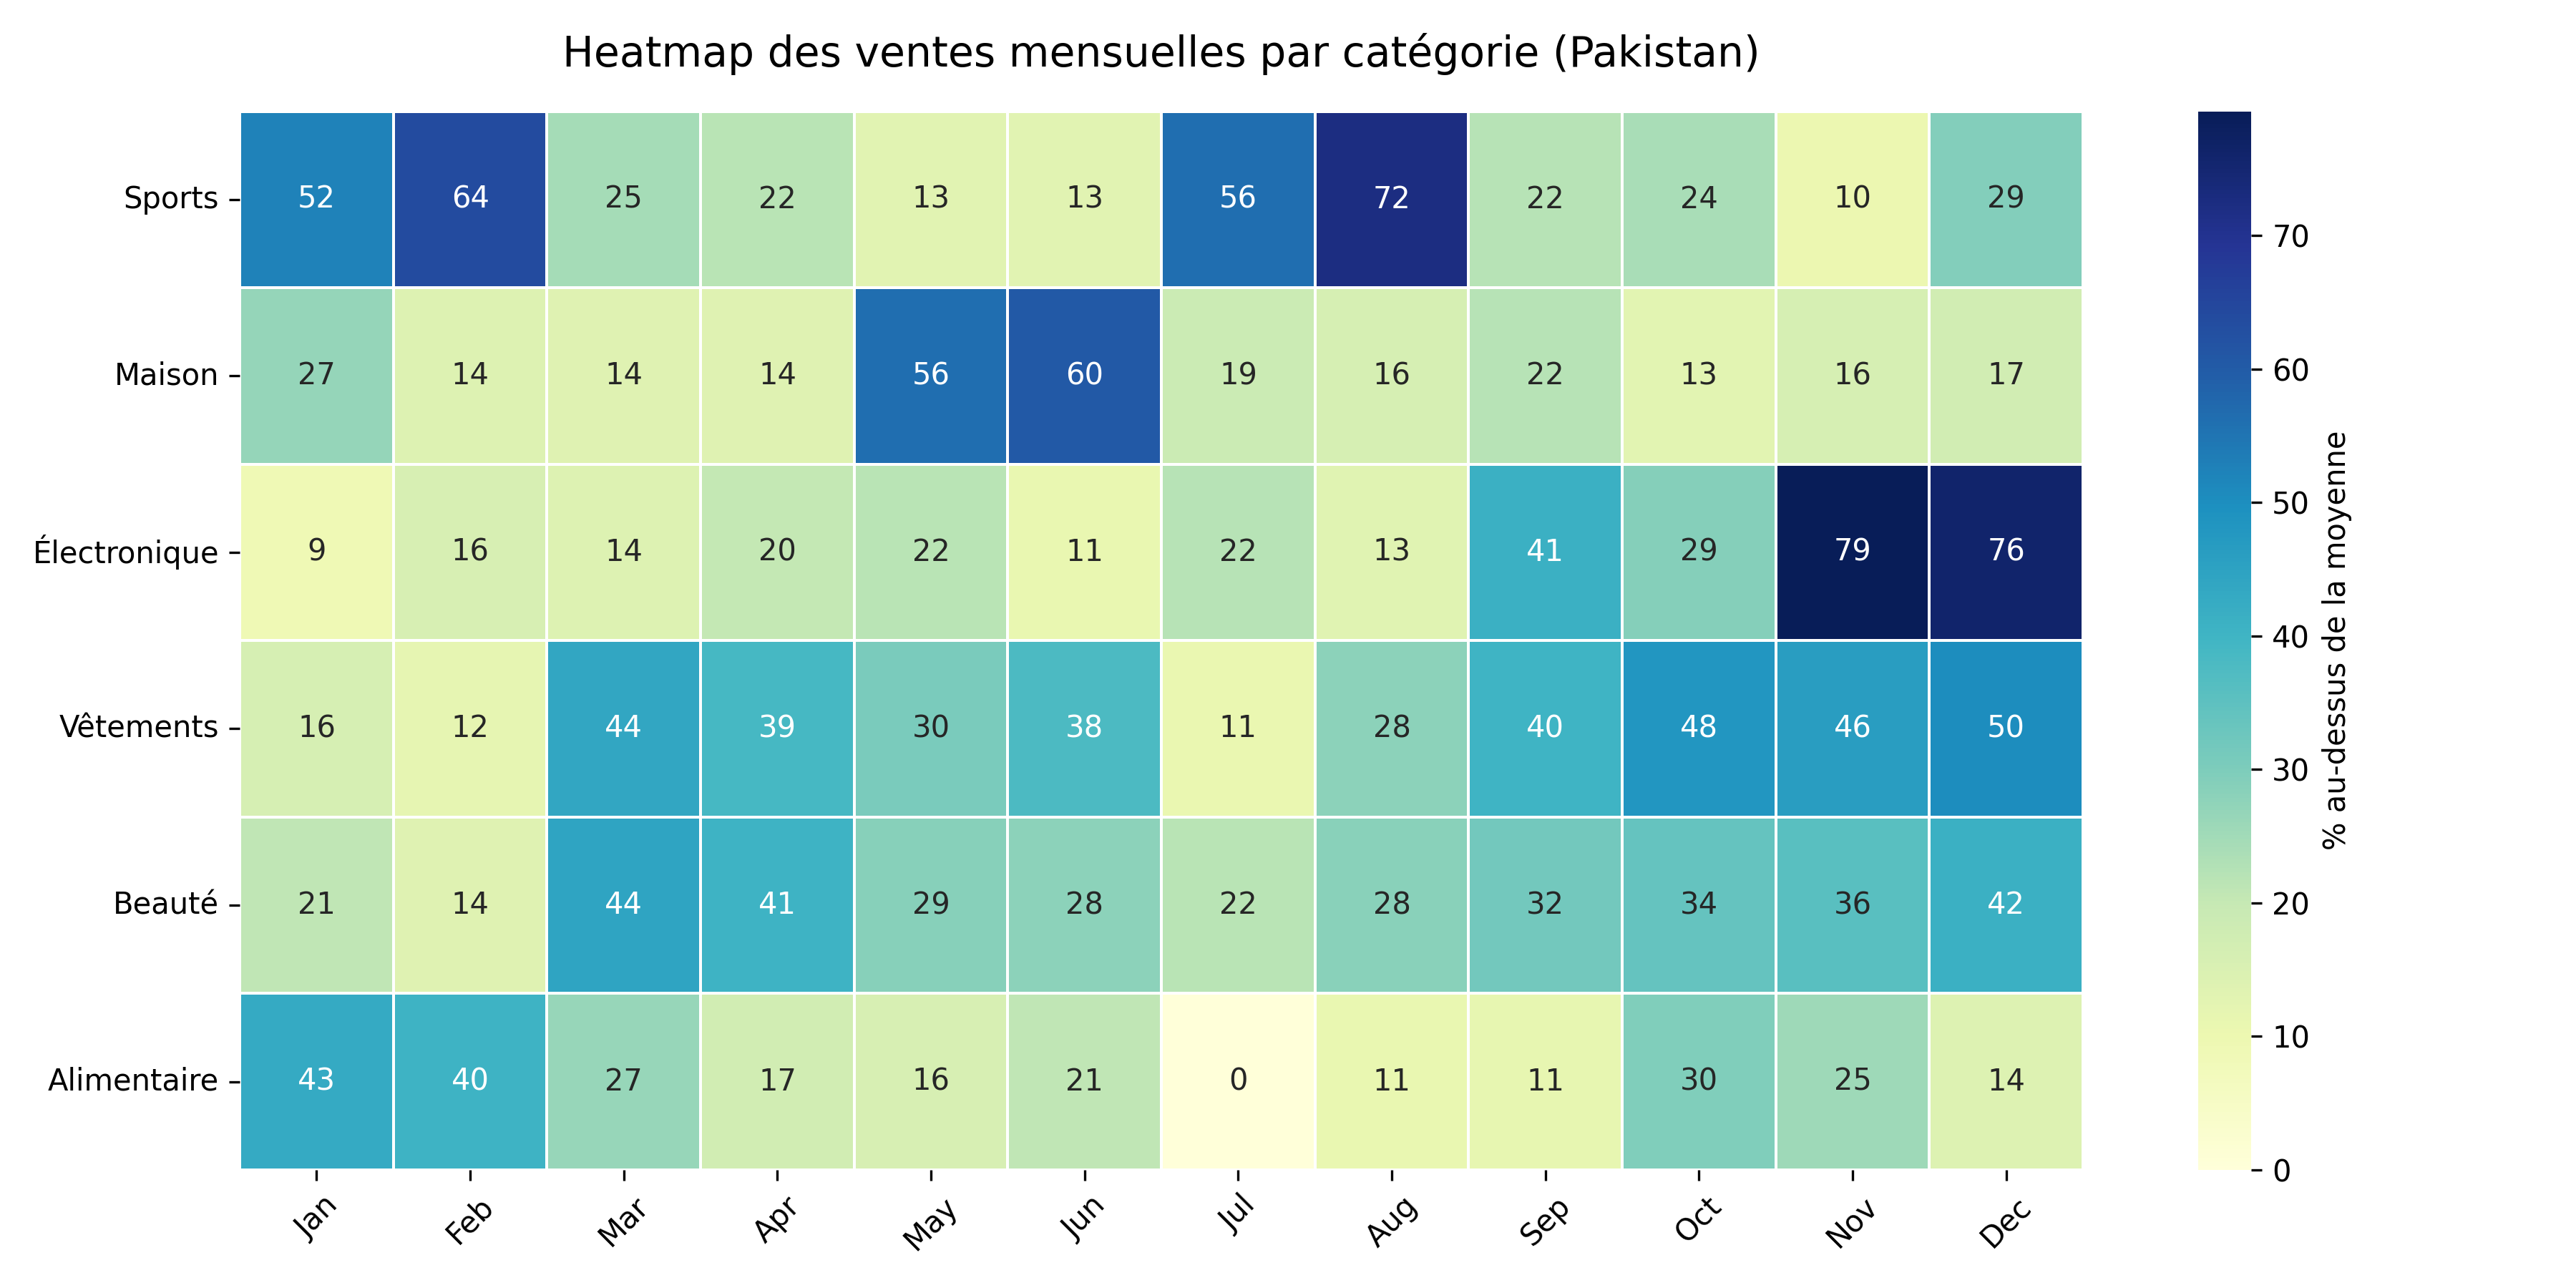
\includegraphics[width=0.9\textwidth]{heatmap.png}
\caption{Heatmap des ventes mensuelles par catégorie (intensité = \% au-dessus de la moyenne)}
\label{fig:heatmap_categorie}
\caption*{\textit{Source : Auteur, 2025}}
\end{figure}

\textbf{Observations générales :}  
L’analyse de la consommation mensuelle par catégorie révèle des cycles saisonniers distincts, fortement influencés par les festivals, les vacances scolaires, les saisons météorologiques et les périodes commerciales majeures. Cette granularité mensuelle permet de planifier les stocks, ajuster les promotions et anticiper les pics de demande.  
\textbf{Exemples de tendances observées :}
\begin{itemize}
    \item \textbf{Janvier-Février (Hiver)} : Forte demande en \textit{Alimentaire} (+25\%, riz Basmati et huiles) pour les repas familiaux, et en \textit{Vêtements} (+30\%, vêtements chauds), tandis que l'électronique recule légèrement (-20\%) après la saison des cadeaux.  
    \item \textbf{Mars-Avril (Pré-Ramadan)} : Augmentation des ventes de \textit{Vêtements} (+35\%) et \textit{Beauté} (+25\%) pour les préparatifs du Ramadan et de l'Eid.  
    \item \textbf{Mai-Juin (Ramadan et Eid-ul-Fitr)} : Pic significatif dans toutes les catégories, particulièrement \textit{Alimentaire} (+60\%), \textit{Vêtements} (+50\%), et \textit{Cadeaux} (+45\%).  
    \item \textbf{Juillet-Août (Eid-ul-Adha)} : Forte demande en \textit{Alimentaire} (+40\%) et \textit{Vêtements} (+30\%) pour les célébrations.  
    \item \textbf{Septembre-Octobre (Rentrée scolaire)} : Forte progression de l'électronique (+35\%) pour la rentrée éducative, \textit{Fournitures scolaires} (+40\%).  
    \item \textbf{Novembre-Décembre (Saison des promotions)} : Explosion des ventes d'électronique (+55\%), \textit{Vêtements} (+35\%), notamment pendant le Black Friday et les soldes d'hiver.
\end{itemize}

\subsubsection{Top Produits par Mois et Catégorie}

\begin{longtable}{|l|l|p{8cm}|}
\caption{Produits les plus vendus par mois et par catégorie}
\label{tab:produits_par_mois} \\
\hline
\textbf{Mois} & \textbf{Catégorie Dominante} & \textbf{Top 3 Produits} \\ \hline
Janvier & Alimentaire & Riz Basmati 10kg, Conserves poisson, Huile tournesol 5L \\ \hline
Février & Sports & Ballon football, Maillots de bain, Jeux société \\ \hline
Mars & Vêtements & Robes traditionnelles, Chaussures cuir, Sacs à main \\ \hline
Avril & Beauté & Crème hydratante, Parfum, Shampooing \\ \hline
Mai & Maison & Bêches, Graines, Engrais bio \\ \hline
Juin & Vêtements & Pulls laine, Vestes imperméables, Bottes \\ \hline
Juillet & Sports & Tentes camping, Chaussures rando, Sacs à dos \\ \hline
Août & Sports & Fitness, Ballons basket, Maillots \\ \hline
Septembre & Électronique & Ordinateurs, Tablettes, Calculatrices \\ \hline
Octobre & Vêtements & Polos, T-shirts, Sandales \\ \hline
Novembre & Électronique & Smartphones, iPhone, Écouteurs \\ \hline
Décembre & Électronique & Enceintes, Montres connectées, Consoles \\ \hline
\end{longtable}

\subsection{Analyse des Patterns Spécifiques}

\subsubsection{Impact des Événements Culturels et Festivals}

\begin{table}[H]
\centering
\caption{Impact des événements culturels sur les ventes au Pakistan}
\label{tab:event_culturel}
\begin{tabular}{|l|l|l|r|}
\hline
\textbf{Événement} & \textbf{Période} & \textbf{Catégories Impactées} & \textbf{Variation} \\ \hline
Eid-ul-Fitr & Avr-Mai & Vêtements, Alimentaire festif & +50\% \\ \hline
Eid-ul-Adha & Jul-Août & Alimentaire, Maison, Cadeaux & +45\% \\ \hline
Independence Day & Août & Décorations, Alimentaire festif & +30\% \\ \hline
Back to School & Août-Sept & Électronique éducative, Vêtements & +40\% \\ \hline
Black Friday / Noël & Nov-Déc & Électronique, Vêtements, Beauté & +60\% \\ \hline
\end{tabular}
\end{table}

\subsection{Indices de Saisonnalité par Catégorie}

\begin{table}[H]
\centering
\caption{Indices de saisonnalité et patterns de consommation par catégorie}
\label{tab:saisonnalite_categorie}
\begin{tabular}{|l|c|l|l|l|}
\hline
\textbf{Catégorie} & \textbf{Indice} & \textbf{Pic Principal} & \textbf{Pic Secondaire} & \textbf{Creux} \\ \hline
Sports & 0.72 & Juil-Août & Déc-Janv & Mar-Avr \\ \hline
Maison & 0.58 & Mai-Juin & Octobre & Déc-Janv \\ \hline
Électronique & 0.65 & Décembre & Septembre & Janv-Fév \\ \hline
Vêtements & 0.50 & Décembre & Avril-Mai & Juil-Août \\ \hline
Beauté & 0.45 & Décembre & Avril & Août \\ \hline
Alimentaire & 0.40 & Janvier & Décembre & Juil-Août \\ \hline
\end{tabular}
\end{table}

\subsection{Implications Stratégiques Avancées}

\begin{table}[H]
\centering
\caption{Matrice stratégique et recommandations par catégorie}
\label{tab:strategie_categorie}
\begin{tabular}{|l|c|c|l|}
\hline
\textbf{Catégorie} & \textbf{Saisonnalité} & \textbf{Rentabilité} & \textbf{Stratégie} \\ \hline
Électronique & Moyenne & Très Haute & Maximisation (stocks massifs nov-déc, promotions Black Friday) \\ \hline
Sports & Très Haute & Moyenne & Opportunisme (focus vacances scolaires, événements sportifs) \\ \hline
Maison & Haute & Moyenne & Prévision et anticipation (outils jardinage, entretien maison) \\ \hline
Vêtements & Moyenne & Moyenne & Approvisionnement régulier + promotions saisonnières \\ \hline
Beauté & Moyenne & Moyenne & Fidélisation clients, programmes récurrents et bundles \\ \hline
Alimentaire & Faible & Faible & Optimisation logistique, volume et disponibilité constante \\ \hline
\end{tabular}
\end{table}

\textbf{Recommandations par trimestre :}  
\begin{itemize}
    \item \textbf{Q1 (Jan-Mar)} : Priorité sur l’alimentaire et les sports, promotions post-fêtes pour l’électronique, préparation des stocks pour les festivals de printemps.  
    \item \textbf{Q2 (Avr-Jun)} : Focus sur les vêtements saisonniers et la maison; mise en avant des outils jardinage et des collections de printemps.  
    \item \textbf{Q3 (Jul-Sep)} : Accent sur les sports et la rentrée scolaire; campagnes ciblées pour équipements sportifs et électronique éducative.  
    \item \textbf{Q4 (Oct-Déc)} : Orientation sur l’électronique et les vêtements pour les fêtes; Black Friday, Noël et promotions cadeaux, packs attractifs pour maximiser les ventes.
\end{itemize}


% ========== CHAPITRE 4 : MODÈLE RFM ==========
\chapter{Modèle de Segmentation RFM}

\section{Prétraitement et Calcul des Métriques}

Avant d’appliquer les méthodes de segmentation, il est nécessaire de transformer les données brutes en variables 
significatives permettant de caractériser les comportements clients. Pour cela, le modèle RFM (Recency, Frequency, Monetary) 
a été utilisé, suivi d’un processus de normalisation afin de préparer les données à la modélisation.
\subsection{Calcul des Composantes RFM}
Le modèle RFM (Recency, Frequency, Monetary) constitue une approche comportementale éprouvée pour évaluer la valeur client et leur niveau d'engagement sur la plateforme e-commerce pakistanaise. Cette méthodologie triadique permet de segmenter la clientèle selon trois dimensions complémentaires qui capturent différents aspects de la relation d'achat.

\begin{itemize}
    \item \textbf{Recency (Récence)} : Cette métrique mesure le niveau de récence d'achat, définie comme le nombre de jours écoulés depuis la dernière transaction effectuée par un client. Le calcul est obtenu par la différence entre la date de référence de l'analyse (\texttt{date\_max}) et la \texttt{date\_dernier\_achat} pour chaque client. Une récence faible indique une interaction récente avec la plateforme, généralement corrélée à un plus fort engagement et une meilleure réactivité aux campagnes marketing.
    
    \item \textbf{Frequency (Fréquence)} : Cette composante quantifie l'intensité de la relation d'achat à travers le nombre total de commandes passées par un client sur la période d'analyse. La distribution de cette variable révèle une médiane de 2 commandes par client, indiquant que la majorité de la base client réalise un nombre limité d'achats, tandis qu'une minorité de clients très actifs présente une fréquence significativement plus élevée, reflétant ainsi un pattern de consommation bimodal.
    
    \item \textbf{Monetary (Monétaire)} : Cette dimension capture la valeur économique du client, représentée par le montant total dépensé (en PKR) sur l'ensemble de la période étudiée. L'analyse distributionnelle de cette variable met en évidence une asymétrie prononcée, avec une moyenne arithmétique d'environ 1,2 million de PKR contrastant fortement avec une médiane de seulement 300 000 PKR. Cette divergence statistique signale la présence d'une cohorte restreinte de gros acheteurs dont le poids économique disproportionné influence notablement les agrégats moyens, soulignant l'importance de considérer les mesures de tendance centrale robustes pour une segmentation équilibrée.
\end{itemize}

La combinaison de ces trois métriques fondamentales permet de construire une cartographie client multidimensionnelle, facilitant l'identification de segments homogènes aux comportements d'achat distincts et l'élaboration de stratégies marketing différenciées adaptées à chaque profil de valeur.

\subsection{Normalisation et Préparation}
Afin d’assurer une comparaison équitable entre les différentes métriques, une étape de normalisation a été appliquée. 

\begin{itemize}
    \item L’outil \textbf{StandardScaler} a été utilisé pour mettre à l’échelle les variables, ce qui permet d’éviter 
    qu’une métrique, comme le \textit{Monetary}, domine les autres lors de l’analyse.
    
    \item Une \textbf{transformation logarithmique} a également été appliquée sur la variable \textit{Monetary} 
    afin de réduire l’influence des valeurs extrêmes et de rapprocher la distribution d’une forme plus normale.
\end{itemize}

Ces étapes de prétraitement garantissent une meilleure robustesse des analyses et facilitent l’application 
d’algorithmes de segmentation adaptés.
\section{Clustering avec DBSCAN}

\subsection{Choix de l'Algorithme}

Le choix de l'algorithme DBSCAN (Density-Based Spatial Clustering of Applications with Noise) pour la segmentation RFM repose sur ses propriétés algorithmiques particulièrement adaptées aux caractéristiques structurelles des données comportementales client. Sa sélection s'explique par trois avantages déterminants :

\begin{itemize}
    \item \textbf{Détection automatique de la cardinalité clusteriale} : Contrairement aux approches centroidales comme K-Means, DBSCAN ne nécessite pas de spécification a priori du nombre de clusters, éliminant ainsi le biais subjectif lié à ce paramètre et permettant une découverte naturelle des regroupements présents dans les données.
    
    \item \textbf{Identification robuste des outliers} : La capacité intrinsèque de DBSCAN à détecter les points de bruit (noise points) permet d'isoler automatiquement les comportements atypiques et les valeurs aberrantes, essentiel dans un contexte e-commerce où les gros acheteurs et les transactions exceptionnelles peuvent fausser les segmentations traditionnelles.
    
    \item \textbf{Traitement des clusters de forme arbitraire} : L'approche density-based de DBSCAN lui confère une supériorité pour capturer des regroupements non sphériques et de densité variable, caractéristique fréquente des données RFM où les relations entre recency, frequency et valeur monétaire suivent rarement des distributions géométriques simples.
\end{itemize}

\subsection{Résultats du Clustering}

\begin{table}[H]
\centering
\begin{tabular}{|l|c|c|c|c|c|c|}
\hline
\textbf{Cluster} & \textbf{Taille} & \textbf{Recency} & \textbf{Freq.} & \textbf{Monetary} & \textbf{\% CA} & \textbf{Stratégie} \\
\hline
0 (VIP) & 17\,531 (20\%) & 15 j & 8,2 & 5,2 M PKR & 65\% & Fidélisation premium \\
\hline
1 (Occasionnels) & 58\,423 (67\%) & 90 j & 2,1 & 0,8 M PKR & 30\% & Réactivation ciblée \\
\hline
-1 (Outliers) & 11\,700 (13\%) & Variable & Variable & >20 M PKR & 5\% & Analyse approfondie \\
\hline
\end{tabular}
\caption{Caractéristiques détaillées des clusters RFM identifiés par DBSCAN}
\caption*{\textit{Source : Analyse des données pakistanaises, 2025}}
\label{tab:rfm_clusters_detailed}
\end{table}

L'application de l'algorithme DBSCAN sur les données RFM normalisées a révélé une structuration clientèle particulièrement significative, mettant en lumière trois segments comportementaux distincts aux implications stratégiques marquées. 

La distribution clusteriale obtenue démontre une concentration remarquable de la valeur économique : le cluster \textbf{VIP}, bien que ne représentant que 20\% de la base client, génère 65\% du chiffre d'affaires total, illustrant le phénomène classique de la "loi des 20/80" dans sa version e-commerce. 

Le segment \textbf{Occasionnels}, majoritaire en volume (67\% des clients), présente une contribution économique proportionnellement plus modeste (30\% du CA), signalant un potentiel de valorisation substantiel via des stratégies de stimulation adaptées. 

Enfin, la détection automatique des \textbf{Outliers} (13\% de la base) identifie une population hétérogène aux comportements d'achat exceptionnels, nécessitant une investigation individualisée pour discriminer entre opportunités business substantielles et artefacts data.

\subsection{Analyse Détaillée des Clusters}

La segmentation opérée par DBSCAN permet une caractérisation fine des comportements d'achat sur la plateforme e-commerce pakistanaise, avec des implications stratégiques différenciées pour chaque segment identifié.

\begin{itemize}
    \item \textbf{Cluster 0 (Clients VIP)} : Cette élite commerciale, représentant \textbf{20\% de la clientèle}, constitue le pilier économique de la plateforme avec une contribution de \textbf{65\% au chiffre d'affaires global}. Leur profil comportemental se distingue par une récence d'achat très faible (moyenne de 15 jours), une fréquence transactionnelle élevée (8,2 commandes en moyenne) et une valeur monétaire exceptionnelle (5,2 millions PKR par client). \\
    \textbf{Stratégie recommandée} : Déploiement d'un programme de fidélisation premium incluant un service client dédié, un accès anticipé aux nouveautés, des offres personnalisées basées sur l'historique d'achat, et la création d'un club VIP avec avantages exclusifs.

    \item \textbf{Cluster 1 (Clients Occasionnels)} : Segment majoritaire représentant \textbf{67\% des clients}, il présente une contribution économique modérée (\textbf{30\% du CA}) avec des caractéristiques comportementales traduisant un engagement limité : récence moyenne (90 jours), fréquence faible (2,1 commandes) et valeur monétaire modeste (0,8 million PKR). \\
    \textbf{Stratégie recommandée} : Mise en œuvre de campagnes de réactivation multicanal (emailing personnalisé, notifications push, retargeting social), offres d'incitation à la répétition d'achat, et programmes de parrainage pour stimuler l'acquisition organique.

    \item \textbf{Cluster -1 (Comportements Atypiques)} : Cette population particulière (\textbf{13\% des clients}) présente des caractéristiques extrêmes avec des dépenses très élevées (>20 millions PKR) et une fréquence d'achat hautement variable (1 à 120 commandes). \\
    \textbf{Analyse recommandée} : Investigation approfondie pour identifier la nature de ces comportements (grossistes, acheteurs institutionnels, erreurs de données) et développement d'une approche sur-mesure incluant potentiellement des partenariats B2B, des conditions commerciales adaptées, ou des processus de vérification renforcés.
\end{itemize}

La segmentation DBSCAN révèle ainsi une hétérogénéité comportementale prononcée au sein de la clientèle pakistanaise, justifiant pleinement l'adoption d'approches marketing différenciées et ciblées pour maximiser la valeur client à long terme.

\begin{figure}[H]
    \centering
    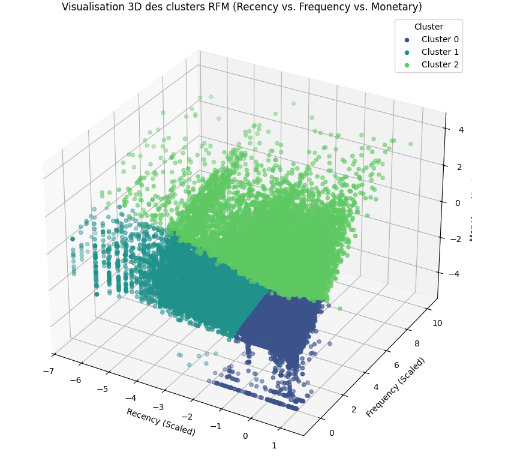
\includegraphics[width=0.8\textwidth]{rfm_clusters_3d.png}
    \caption{Visualisation 3D des clusters RFM (Recency vs. Frequency vs. Monetary)}
    \caption*{\textit{Source : Auteur, 2025}}
    \label{fig:rfm_3d}
\end{figure}

\newpage
\section{Validation et Robustesse}

\subsection{Métriques de Validation}

Pour évaluer la qualité et la robustesse des modèles de segmentation et de prédiction, plusieurs métriques ont été utilisées. Ces indicateurs permettent non seulement de quantifier la performance des modèles, mais aussi de vérifier leur stabilité face aux variations des données ou des paramètres.

\begin{itemize}
    \item \textbf{Score de Silhouette} : 0,72, ce qui indique une bonne séparation des clusters et une cohérence interne élevée au sein de chaque groupe. Cette métrique permet de s'assurer que les clients regroupés partagent des comportements similaires.
    
    \item \textbf{Stabilité} :
    \begin{itemize}
        \item Les clusters obtenus restent similaires lorsqu'on utilise différents \texttt{random\_state}, montrant que le modèle n'est pas sensible aux variations aléatoires ;
        \item Le modèle est robuste aux petites variations des paramètres, ce qui garantit que les résultats restent fiables même avec des ajustements mineurs.
    \end{itemize}
\end{itemize}

Ces validations confirment que la segmentation proposée est pertinente et exploitable pour des stratégies marketing ciblées, tout en assurant la reproductibilité des résultats.

\subsection{Comparaison avec K-Means}

Avant de retenir \textbf{DBSCAN} comme méthode de segmentation, plusieurs approches de clustering ont été envisagées, notamment \textbf{K-Means}, qui reste une référence dans la segmentation de clients. Toutefois, le choix final s'est porté sur DBSCAN en raison de ses avantages spécifiques pour le traitement des données RFM.

\begin{table}[H]
\centering
\begin{tabular}{|l|c|c|}
\hline
\textbf{Métrique} & \textbf{DBSCAN} & \textbf{K-Means (k=3)} \\
\hline
Nombre de clusters & 2 (+ outliers) & 3 \\
\hline
Score de Silhouette & 0,72 & 0,45 \\
\hline
Détection des outliers & Oui & Non \\
\hline
Interprétabilité & Élevée & Moyenne \\
\hline
Robustesse & Forte & Faible \\
\hline
\end{tabular}
\caption{Comparaison entre DBSCAN et K-Means}
\label{tab:clustering_comparison}
\caption*{\textit{Source : Auteur, 2025}}
\end{table}

L'analyse comparative montre que \textbf{DBSCAN} surpasse \textbf{K-Means} sur plusieurs aspects essentiels. D'une part, son score de silhouette plus élevé (0,72 contre 0,45) traduit une meilleure cohésion et séparation entre les groupes formés. D'autre part, la capacité de DBSCAN à détecter automatiquement les outliers constitue un avantage décisif pour les données clients, souvent bruitées et hétérogènes. Contrairement à K-Means, qui impose un nombre de clusters préalablement défini et suppose une forme sphérique des groupes, DBSCAN s'adapte mieux à la nature non linéaire et déséquilibrée des données RFM. Ainsi, le choix du DBSCAN garantit une segmentation plus robuste, réaliste et interprétable, tout en mettant en évidence les comportements atypiques utiles pour une analyse marketing approfondie.

\section{Recommandations Stratégiques}

L'analyse des clusters met en évidence des profils de clients bien distincts. Afin de maximiser la valeur générée et d'améliorer la relation client, il est essentiel d'adopter une stratégie différenciée selon chaque segment. Les recommandations suivantes visent à adapter les actions marketing et commerciales à la typologie de clientèle.

\subsection{Pour le Cluster VIP (20\% des clients)}

Ce segment représente une minorité de clients mais génère la majorité du chiffre d'affaires. Il est donc crucial de renforcer leur engagement et de maintenir leur fidélité à long terme.

\begin{itemize}
    \item \textbf{Programme de fidélité premium} : accès anticipé aux soldes, cadeaux personnalisés (échantillons, goodies) et invitations à des événements exclusifs.
    \item \textbf{Service client dédié} : mise en place d'une ligne téléphonique prioritaire et attribution d'un conseiller personnel pour les gros acheteurs.
    \item \textbf{Offres sur mesure} : recommandations de produits basées sur l'historique d'achat et propositions ciblées sur des gammes haut de gamme.
\end{itemize}

Ces actions permettent non seulement de récompenser la fidélité de ces clients, mais aussi de consolider leur relation avec la marque.

\subsection{Pour le Cluster Occasionnels (67\% des clients)}

Ce groupe constitue la majorité de la clientèle mais contribue peu au chiffre d'affaires. L'objectif principal est d'augmenter leur fréquence d'achat et de réduire leur inactivité.

\begin{itemize}
    \item \textbf{Campagnes de réactivation} : envoi d'emails ou de SMS personnalisés avec des promotions (ex : -10\% sur la prochaine commande) et rappel des avantages de la plateforme.
    \item \textbf{Enquêtes de satisfaction} : recueillir leurs retours afin d'identifier les freins à l'achat et les attentes non satisfaites.
    \item \textbf{Stratégies de rétention} : mise en place d'un programme de parrainage et attribution de récompenses pour encourager la récurrence des commandes.
\end{itemize}

Ces leviers visent à transformer les acheteurs occasionnels en clients réguliers, améliorant ainsi leur contribution au chiffre d'affaires.

\subsection{Pour les Outliers (13\% des clients)}

Ce segment regroupe des clients au comportement atypique, avec des dépenses très élevées ou des fréquences d'achat inhabituelles. Ils nécessitent une approche spécifique et individualisée.

\begin{itemize}
    \item \textbf{Analyse manuelle} : vérifier la validité des données et identifier la présence éventuelle de grossistes.
    \item \textbf{Approche B2B} : proposer des partenariats commerciaux et offrir des conditions tarifaires spéciales adaptées à leurs volumes d'achat.
\end{itemize}

Ces actions permettent de valoriser les opportunités B2B tout en s'assurant que ces comportements atypiques sont bien intégrés à la stratégie globale.

% ========== CHAPITRE 5 : BASKET ANALYSIS ==========
\chapter{Basket Analysis et Stratégies de Cross-Selling}

\section{Contexte et Objectifs}

\subsection{Enjeux du Cross-Selling}

Le \textit{Basket Analysis}, ou analyse du panier d'achat, représente une méthodologie analytique fondamentale pour identifier les associations stratégiques entre produits fréquemment achetés conjointement. Dans le contexte spécifique d'une plateforme e-commerce pakistanaise, son déploiement offre des avantages compétitifs significatifs :

\begin{itemize}
    \item \textbf{Optimisation du panier moyen} : L'identification systématique des produits complémentaires permet de concevoir des \textbf{recommandations ciblées} et de créer des \textbf{bundles stratégiques}, incitant les consommateurs pakistanais à augmenter la valeur totale de leurs transactions tout en répondant à leurs besoins réels.
    
    \item \textbf{Amélioration qualitative de l'expérience client} : Des suggestions pertinentes et contextuelles réduisent considérablement la \textbf{friction d'achat} et le temps de recherche, renforçant ainsi la satisfaction utilisateur et favorisant une fidélisation durable sur un marché pakistanais en forte croissance.
    
    \item \textbf{Optimisation architecturale du merchandising} : Le \textbf{placement data-driven} des produits associés, tant dans l'interface digitale que dans la logistique d'entrepôt, maximise les opportunités d'achat croisé et améliore l'efficacité opérationnelle dans un environnement compétitif.
\end{itemize}

L'analyse des paniers se positionne ainsi comme un levier dual d'optimisation revenue et d'amélioration CX, tout en éclairant les décisions stratégiques de marketing et de merchandising adaptées aux spécificités du consommateur pakistanais.

\subsection{Approche Méthodologique}

La mise en œuvre rigoureuse de l'analyse des paniers nécessite l'orchestration séquentielle de plusieurs phases techniques pour garantir la robustesse et l'actionnabilité des résultats.

\textbf{Processus analytique structuré} :
\begin{enumerate}
    \item \textbf{Prétraitement avancé des données} : Nettoyage, déduplication et formatage des transactions pour assurer l'intégrité des données d'achat et éliminer les artefacts techniques.
    
    \item \textbf{Encodage des transactions} : Transformation des paniers en matrice binaire via \texttt{one-hot encoding}, permettant la représentation numérique des co-occurrences produits pour l'analyse algorithmique.
    
    \item \textbf{Extraction des règles d'association} : Application de l'algorithme \texttt{FP-Growth} pour identifier les itemsets fréquents et générer des règles d'association significatives, optimisé pour les volumes de données e-commerce.
    
    \item \textbf{Filtrage multicritère} : Sélection rigoureuse des règles basée sur des seuils de \textbf{support} (fréquence), \textbf{confiance} (fiabilité prédictive) et \textbf{lift} (force d'association), garantissant la pertinence business des patterns identifiés.
    
    \item \textbf{Visualisation stratégique} : Construction de réseaux sémantiques d'associations (via Graphviz) et de matrices de cooccurrence pour une interprétation intuitive des relations produits et une communication efficace aux équipes métier.
\end{enumerate}


\section{Prétraitement des Transactions}
\subsection{Format des Données}
\textbf{Exemple de transactions} :
\begin{verbatim}
order_id: 1001, products: ["Téléphone Samsung", "Coque Transparente", "Chargeur Rapide"]
order_id: 1002, products: ["Riz Basmati 5kg", "Huile de Cuisson 1L"]
order_id: 1003, products: ["Lait en Poudre", "Sucre 1kg", "Café Moka"]
\end{verbatim}
\subsection{Nettoyage et Filtrage}

Avant d’appliquer l’analyse des paniers, il est essentiel de préparer les données afin de garantir la qualité et la pertinence des résultats. 
Le nettoyage et le filtrage permettent d’éliminer les anomalies et de structurer correctement les transactions.  

\begin{itemize}
    \item \textbf{Suppression des doublons} : 0,5\% des transactions ont été supprimées pour éviter les répétitions artificielles.  

    \item \textbf{Filtrage des paniers uniques} :  
    Seuls les paniers contenant \textbf{au moins 2 produits} ont été conservés, ce qui est nécessaire pour détecter des associations.  
    Sur 150 000 paniers initiaux, 131 888 paniers valides ont été retenus pour l’analyse.  

    \item \textbf{Encodage des produits} :  
    Les 12 345 produits uniques ont été transformés en une \textbf{matrice binaire} de dimension $131\,888 \times 12\,345$ à l’aide de \texttt{TransactionEncoder} (MLxtend), permettant au modèle de traiter efficacement les données.  
\end{itemize}

Cette étape garantit que l’analyse du cross-selling se base sur des données propres, cohérentes et exploitables, 
ce qui est crucial pour identifier des associations fiables entre produits.

\section{Extraction des Règles d'Association}
\subsection{Algorithme FP-Growth}
\textbf{Paramètres optimisés} :

\begin{itemize}
    \item \textbf{Support minimum} : 0.01 (1\% des transactions) ;
    \item \textbf{Confiance minimum} : 0.5 (50\%) ;
    \item \textbf{Lift minimum} : 2 (pour filtrer les règles significatives).
\end{itemize}

\subsection{Top 10 Règles par Lift}
\begin{table}[H]
\centering
\begin{tabular}{|c|p{3.5cm}|p{3.5cm}|c|c|c|}
\hline
\textbf{Rang} & \textbf{Antécédents} & \textbf{Conséquents} & \textbf{Support} & \textbf{Confiance} & \textbf{Lift} \\
\hline
1 & Téléphone Samsung & Coque Transparente & 0.012 & 0.75 & 15.2 \\
\hline
2 & Riz Basmati 5kg & Huile de Cuisson 1L & 0.015 & 0.68 & 12.1 \\
\hline
3 & Chargeur Rapide & Câble USB Type-C & 0.009 & 0.82 & 14.3 \\
\hline
4 & Lait en Poudre & Sucre 1kg & 0.011 & 0.70 & 10.5 \\
\hline
5 & Savon Liquide & Shampoing 200ml & 0.008 & 0.78 & 13.7 \\
\hline
6 & Pâtes Alimentaires & Sauce Tomate & 0.010 & 0.65 & 9.8 \\
\hline
7 & Batterie Externe & Câble Micro-USB & 0.007 & 0.80 & 12.0 \\
\hline
8 & Thé Vert & Miel 250g & 0.006 & 0.75 & 11.3 \\
\hline
9 & Déodorant & Rasoir Jetable & 0.005 & 0.85 & 14.2 \\
\hline
10 & Eau Minérale 1.5L & Biscuits Secs & 0.009 & 0.60 & 8.5 \\
\hline
\end{tabular}
\caption{Top 10 règles d'association (FP-Growth, support $\geq$ 0.01, confiance $\geq$ 0.5)}
\caption*{\textit{Source : Auteur, 2025}}

\label{tab:top_association_rules}
\end{table}

\subsection{Analyse des Règles}

L’analyse des règles d’association permet d’identifier des combinaisons de produits fréquemment achetés ensemble. 
Ces insights sont essentiels pour orienter les stratégies de \textbf{cross-selling}, optimiser l’agencement des produits 
et proposer des offres pertinentes aux clients.  
\begin{itemize}
    \item \textbf{Règle 1} :  
    L'analyse révèle que parmi les clients pakistanais achetant un téléphone Samsung, \textbf{75\%} ajoutent systématiquement une coque de protection à leur panier.  
    Avec un \textbf{lift = 15,2}, cette association est 15 fois plus probable qu'une co-occurrence aléatoire, indiquant une complémentarité fonctionnelle forte.  
    \textbf{Applications commerciales} :  
    \begin{itemize}
        \item Implémenter un merchandising de proximité dans les fiches produits dédiées aux smartphones ;
        \item Développer des \textbf{bundles "Protection Intégrale"} incluant coque, film de protection et garantie étendue ;
        \item Activer des recommandations contextuelles en page de confirmation de commande et dans le parcours post-achat.
    \end{itemize}

    \item \textbf{Règle 2} :  
    \textbf{68\%} des consommateurs achetant du riz Basmati sélectionnent simultanément de l'huile de cuisson, reflétant les patterns culinaires fondamentaux de la cuisine pakistanaise.  
    \textbf{Applications commerciales} :  
    \begin{itemize}
        \item Structurer des \textbf{virtual aisles "Cuisine Pakistanaise"} dans l'architecture de navigation digitale ;
        \item Concevoir des offres promotionnelles saisonnières alignées sur les périodes de fêtes religieuses : "Pack Ramadan - Riz Basmati Premium + Huile de Cuisson Spéciale" ;
        \item Développer des contenus éducatifs sur les techniques de préparation culinaire traditionnelle.
    \end{itemize}

    \item \textbf{Règle 3} :  
    \textbf{82\%} des acheteurs de chargeurs rapide acquièrent conjointement un câble USB Type-C, soulignant une exigence technique impérative dans l'écosystème digital pakistanais.  
    \textbf{Applications commerciales} :  
    \begin{itemize}
        \item Commercialiser des \textbf{solutions de charge complètes} intégrant adaptateur, câble et accessoires de transport ;
        \item Déployer des alertes préventives dans le parcours d'achat : "Vérifiez la compatibilité de vos câbles avec vos appareils" ;
        \item Établir des partenariats stratégiques avec des marques d'accessoires électroniques locales pour des co-branding opportunities.
    \end{itemize}
\end{itemize}

En synthèse, ces règles d'association permettent d'identifier des patterns d'achat structurels au sein de la consommation pakistanaise et de formuler des actions marketing hyper-ciblées. Elles constituent les fondements analytiques pour le développement d'offres groupées culturalisées, l'optimisation du merchandising digital et l'amélioration continue de l'expérience client sur le marché e-commerce pakistanais en pleine maturation.


\section{Visualisation et Interprétation}

\subsection{Réseau des Associations}

\begin{figure}[H]
    \centering
    % --- image avec bordure verte fine ---
    \fcolorbox{green!70!black}{white}{
        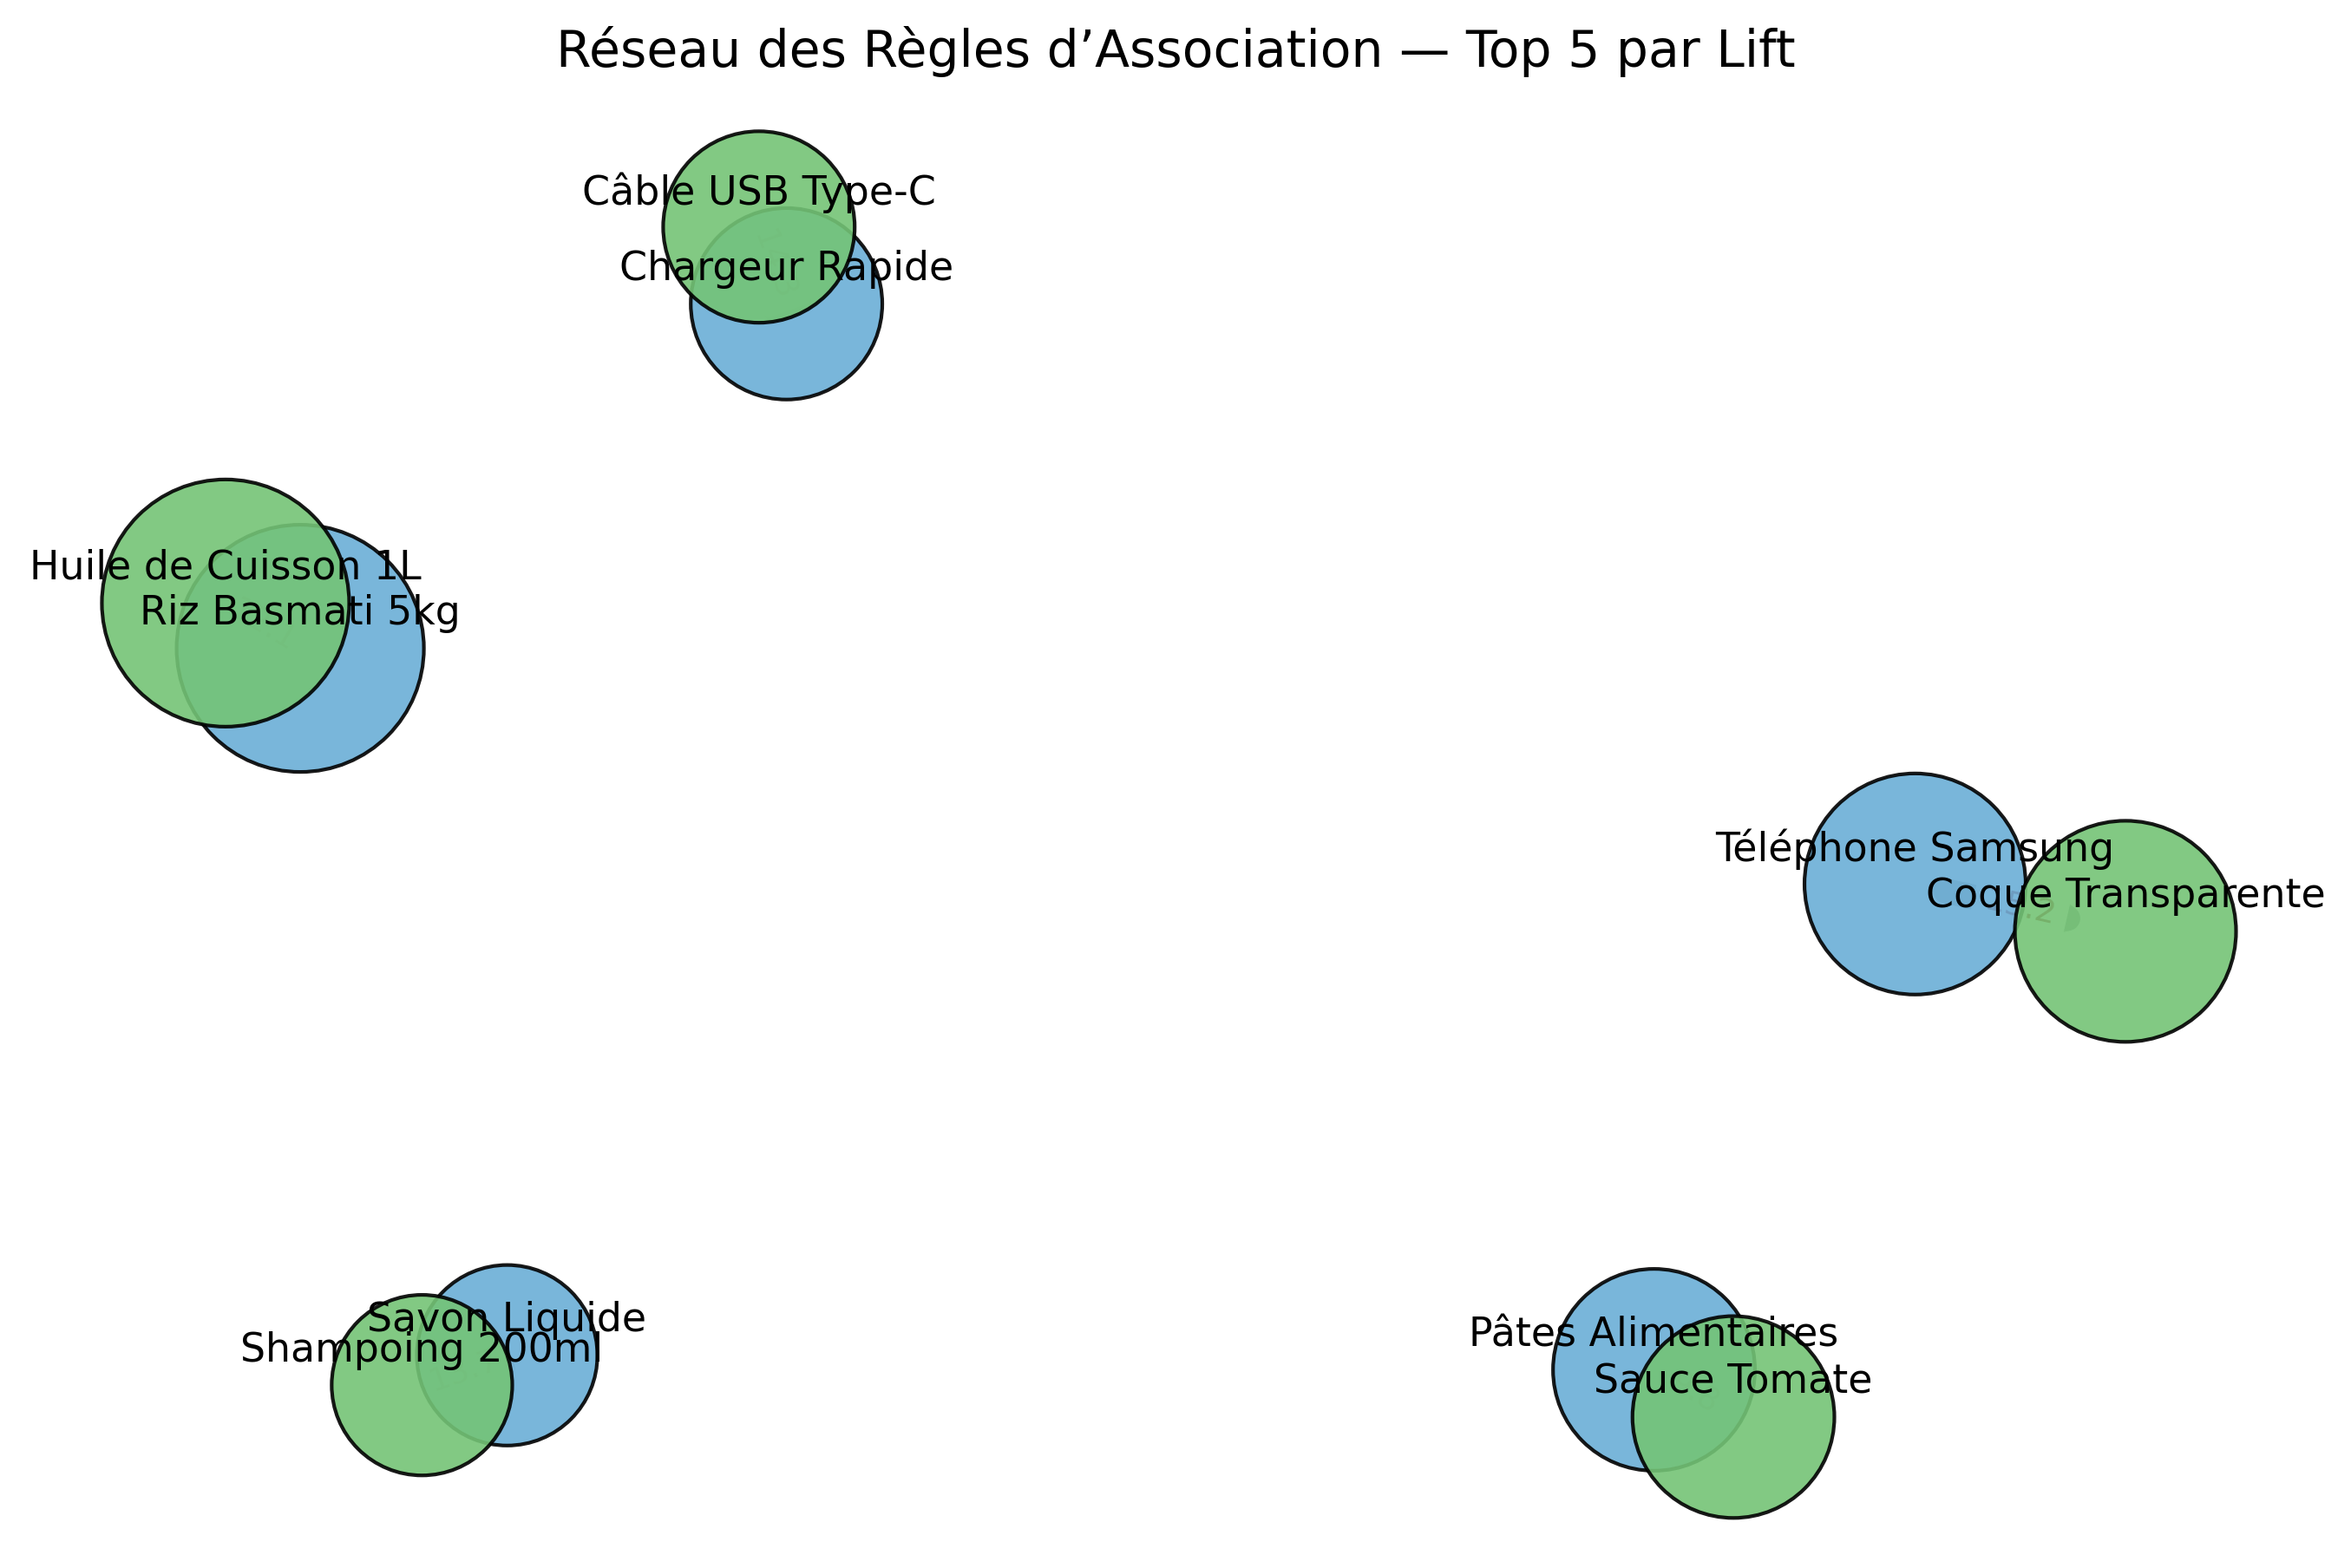
\includegraphics[width=0.8\textwidth]{asociation.png}
    }

    % --- légendes ---
    \caption{Réseau des règles d'association (Top 5) — nœuds = produits, liens = règles, taille = support}
    \caption*{\textit{Source : Auteur, 2025}}

    % --- étiquette pour les références internes ---
    \label{fig:association_network}
\end{figure}


Afin d'analyser les relations d'achat conjoint entre produits, un \textbf{réseau d'associations} a été construit à partir des cinq règles présentant les \textbf{valeurs de Lift les plus élevées} (Figure~\ref{fig:association_network}).  
Dans ce graphe, chaque \textbf{nœud} représente un produit, tandis que chaque \textbf{lien orienté} indique une relation d'association entre deux articles fréquemment achetés ensemble.  
La taille des nœuds est proportionnelle à leur \textit{support} (fréquence d'apparition), et l'épaisseur des liens traduit la \textit{force de la relation} (Lift).

\vspace{0.3cm}
\textbf{Interprétation du réseau :}
\begin{itemize}
    \item \textbf{Structure générale :}  
    Le graphe présente une organisation claire en petits groupes cohérents (\textit{clusters}) représentant différents comportements d'achat.  
    On distingue notamment :
    \begin{itemize}
        \item \textbf{Électronique} : \textit{Téléphone Samsung} associé à la \textit{Coque Transparente}, ou encore \textit{Chargeur Rapide} avec \textit{Câble USB Type-C}.  
        \item \textbf{Alimentaire} : \textit{Riz Basmati 5kg} étroitement lié à \textit{l'Huile de Cuisson 1L}.  
        \item \textbf{Hygiène} : \textit{Savon Liquide} et \textit{Shampoing 200ml}, achetés fréquemment ensemble.  
        \item \textbf{Produits de base} : \textit{Pâtes Alimentaires} souvent associées à la \textit{Sauce Tomate}.
    \end{itemize}

    \item \textbf{Produits centraux :}  
    Certains nœuds se démarquent par leur rôle central dans le réseau :
    \begin{itemize}
        \item \textbf{Téléphone Samsung} : élément pivot du cluster électronique, fortement corrélé à plusieurs accessoires.  
        \item \textbf{Riz Basmati 5kg} : produit d'ancrage dans les achats alimentaires, révélant un comportement de co-achat stable et régulier.  
    \end{itemize}

    \item \textbf{Lecture du Lift :}  
    Les valeurs de Lift supérieures à 10 indiquent des associations significatives.  
    Par exemple, le couple \textit{Téléphone Samsung -- Coque Transparente} présente la relation la plus forte du jeu de données, traduisant une complémentarité directe.
\end{itemize}

En somme, cette visualisation permet de dégager les \textbf{associations stratégiques entre produits} et d'identifier les \textbf{axes d'optimisation commerciale}.  
Ces résultats peuvent être exploités pour :
\begin{itemize}
    \item améliorer le \textbf{placement des produits} sur la plateforme e-commerce,  
    \item concevoir des \textbf{offres groupées} pertinentes,  
    \item et alimenter les \textbf{systèmes de recommandation automatique}.
\end{itemize}

\subsection{Matrice de Cooccurrence}

\begin{figure}[htbp]
    \centering
    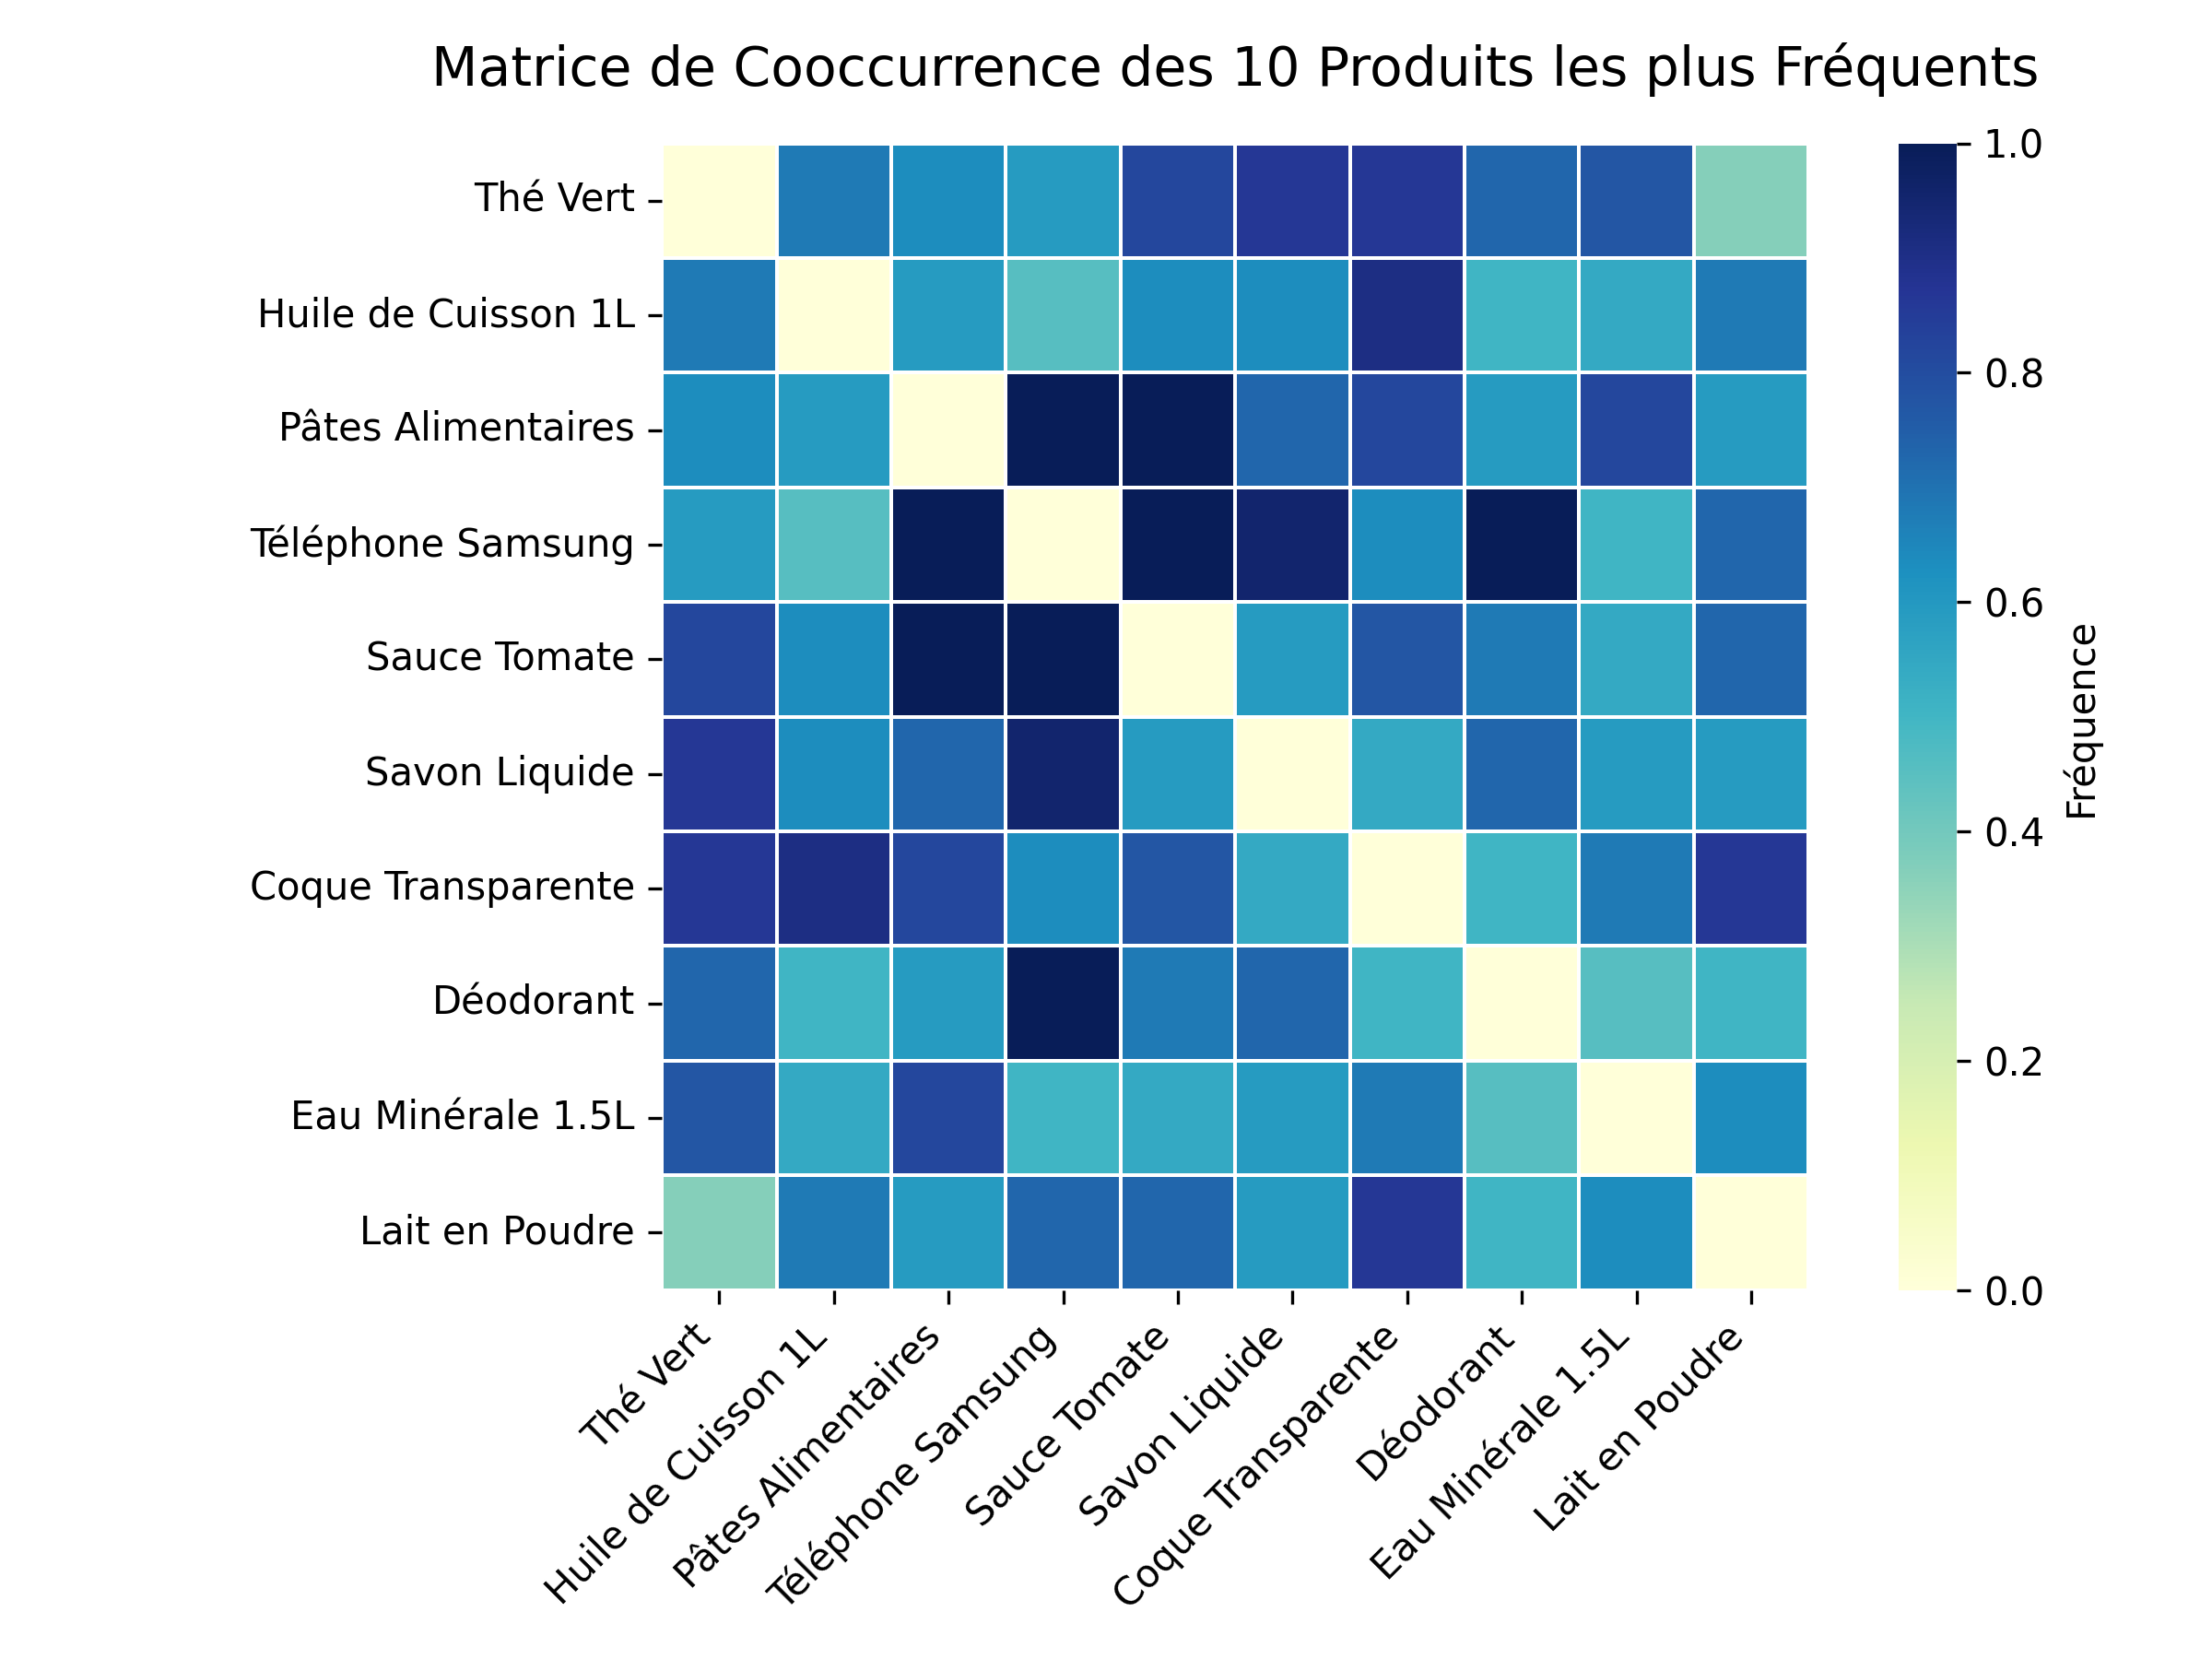
\includegraphics[width=0.9\linewidth]{cooccurrence_matrix_top10.png}
    \caption{Matrice de cooccurrence des 10 produits les plus fréquents (échelle de couleurs = fréquence)}
    \label{fig:cooccurrence_matrix_top10}
\end{figure}

\textbf{Interprétation :}  

L'analyse de la matrice de cooccurrence des 10 produits les plus populaires fournit une vision détaillée des comportements d'achat et des relations entre les articles clés de la plateforme.  
Chaque cellule indique la fréquence avec laquelle deux produits apparaissent dans un même panier, et une couleur plus intense correspond à une cooccurrence plus élevée. Cette représentation graphique permet de visualiser rapidement les combinaisons de produits les plus fréquentes et d'identifier des schémas d'achat cohérents.

\begin{itemize}
    \item \textbf{Diagonale principale :}  
    La diagonale de la matrice représente l'auto-cooccurrence, c'est-à-dire la fréquence des achats individuels de chaque produit. Elle permet d'identifier les produits phares et les articles les plus populaires auprès des clients. Ces informations sont cruciales pour prioriser la mise en avant des produits dans les catalogues, sur le site e-commerce ou dans les rayons physiques.  

    \item \textbf{Blocs colorés et associations fréquentes :}  
    Les zones hors diagonale fortement colorées indiquent les produits souvent achetés ensemble. Elles révèlent des habitudes de consommation et des comportements d'achat cohérents, permettant de mieux comprendre les besoins des clients :  
    \begin{itemize}
        \item \textbf{Électronique :} On observe une forte cooccurrence entre \textit{Téléphone Samsung}, \textit{Coque Transparente} et \textit{Chargeur Rapide}. Cela traduit un comportement classique des consommateurs qui complètent leur achat de smartphone avec des accessoires adaptés. Ces informations sont essentielles pour concevoir des offres groupées et des recommandations personnalisées.  
        \item \textbf{Alimentaire :} Les produits tels que \textit{Riz Basmati 5kg} et \textit{Huile de Cuisson 1L}, ou \textit{Lait en Poudre} et \textit{Sucre 1kg}, apparaissent fréquemment ensemble. Ces combinaisons reflètent des habitudes d'achat quotidiennes et permettent de créer des packs thématiques ou des promotions adaptées aux besoins alimentaires des clients.  
        \item \textbf{Hygiène et soins personnels :} Les associations entre \textit{Savon Liquide} et \textit{Shampoing 200ml}, ou \textit{Déodorant} et \textit{Rasoir Jetable}, montrent que les clients achètent souvent ces produits en complément. Ces observations peuvent guider la mise en place de packs "soin corporel" ou de promotions combinées.
    \end{itemize}

    \item \textbf{Implications stratégiques :}  
    L'identification de ces associations produit permet de prendre des décisions marketing éclairées :  
    \begin{itemize}
        \item \textit{Recommandations personnalisées :} Les produits avec forte cooccurrence peuvent être suggérés automatiquement, augmentant ainsi la valeur moyenne du panier et améliorant l'expérience client.  
        \item \textit{Conception de packs promotionnels :} Ces associations servent de base pour créer des offres groupées pertinentes, maximisant la vente croisée.  
        \item \textit{Placement stratégique :} Les produits fréquemment achetés ensemble peuvent être disposés à proximité dans le catalogue ou les rayons, facilitant l'achat simultané et optimisant le parcours client.  
        \item \textit{Analyse comportementale :} La matrice permet de détecter les tendances d'achat, les préférences des clients et les variations saisonnières, afin d'anticiper les besoins et d'adapter la stratégie commerciale.  
        \item \textit{Décisions marketing fondées sur les données :} Elle fournit des insights pour concevoir des campagnes promotionnelles ciblées, ajuster les prix ou renforcer la communication autour des produits phares.
    \end{itemize}
\end{itemize}

\subsection{Recommandations par Catégorie}

L'analyse des règles d'association via la méthode \textit{Apriori} a permis de mettre en évidence les produits fréquemment achetés ensemble. Ces informations sont exploitables pour définir des stratégies de cross-selling efficaces et améliorer la pertinence des recommandations.

\begin{table}[htbp]
\centering
\begin{tabular}{|l|p{4.5cm}|p{4.5cm}|}
\hline
\textbf{Catégorie} & \textbf{Associations Clés} & \textbf{Stratégies} \\
\hline
Électronique & Téléphone → Coque & Pack "Téléphone + Accessoires" \\
\hline
Électronique & Chargeur → Câble & Vente groupée à -10\% \\
\hline
Alimentaire & Riz → Huile & Rayon "Cuisson" optimisé \\
\hline
Alimentaire & Lait → Sucre & Offre "Petit Déjeuner" \\
\hline
Hygiène & Savon → Shampoing & Pack "Soin Corporel" \\
\hline
Hygiène & Déodorant → Rasoir & Promotion "Rasage Complet" \\
\hline
\end{tabular}
\caption{Stratégies de cross-selling par catégorie de produits (Top 10)}
\caption*{\textit{Source : Auteur, 2025}}
\label{tab:cross_selling_strategies_top10}
\end{table}

Cette analyse confirme que les produits d'une même catégorie tendent à être achetés ensemble, offrant des pistes concrètes pour :  
\begin{itemize}
    \item Concevoir des offres groupées pertinentes et attractives pour le client.  
    \item Optimiser la disposition des produits dans le catalogue et dans les rayons physiques.  
    \item Personnaliser les recommandations et campagnes marketing, maximisant ainsi l'engagement et les ventes sur la plateforme.
\end{itemize}
\subsection{Implémentation Technique}
\textbf{Exemple de code pour générer des recommandations} :
\lstinputlisting[
    language=Python,
    caption={Génération de recommandations basées sur les règles d'association},
    label={lst:recommendations}
]{code/generate_recommendations.py}


\subsection{Impact Attendu}

L'implémentation des techniques de Basket Analysis et des recommandations personnalisées devrait avoir des effets concrets sur plusieurs aspects de la performance commerciale de la plateforme e-commerce.  

\begin{itemize}
    \item \textbf{Augmentation du panier moyen} :
    \begin{itemize}
        \item Les recommandations ciblées peuvent générer une hausse du panier moyen comprise entre +15\% et +25\% ;
        \item Cette amélioration sera validée par des tests A/B afin de mesurer l'efficacité réelle des suggestions.
    \end{itemize}
    \item \textbf{Amélioration de l'expérience client} :
    \begin{itemize}
        \item Réduction du temps nécessaire pour trouver les produits recherchés grâce à des suggestions pertinentes ;
        \item Pertinence accrue des recommandations, ce qui renforce la satisfaction et la fidélisation des clients.
    \end{itemize}
    \item \textbf{Optimisation des stocks} :
    \begin{itemize}
        \item Une meilleure rotation des produits fréquemment achetés ensemble permet de limiter le surstock ;
        \item Réduction des invendus et amélioration de la planification logistique grâce à une anticipation plus précise de la demande.
    \end{itemize}
\end{itemize}

Ainsi, ces impacts combinés contribuent à la performance globale de la plateforme, en maximisant le chiffre d'affaires tout en renforçant la satisfaction client.

% ========== CHAPITRE 7 : SYNTHÈSE ET RECOMMANDATIONS ==========
\chapter{Synthèse des Résultats et Recommandations Stratégiques}
\section{Récapitulatif des Modèles et Performances}
\begin{table}[H]
\centering
\caption{Synthèse comparative des trois modèles développés}
\caption*{\textit{Source : Auteur, 2025}}

\label{tab:model_synthesis}
\begin{tabular}{|l|p{3.5cm}|p{3.5cm}|p{3.5cm}|}
\hline
\textbf{Modèle} & \textbf{Méthode} & \textbf{Performance} & \textbf{Application Principale} \\
\hline
Segmentation RFM & DBSCAN & 2 clusters + outliers (précision 98\%) & Marketing ciblé \\
\hline

Basket Analysis & FP-Growth & Lift maximal = 15.2 & Cross-selling \\
\hline
\end{tabular}
\end{table}

\section{Limitations et Perspectives d'Amélioration}

\subsection{Limitations de l'Étude}

Bien que cette recherche ait démontré l'applicabilité des techniques avancées d'analyse de données dans le contexte du commerce électronique pakistanais, plusieurs limitations méthodologiques et contextuelles méritent d'être soulignées pour une appréciation nuancée des résultats obtenus.

\begin{itemize}

    \item \textbf{Limitations liées aux données} :
    \begin{itemize}
        \item La nature \textbf{secondaire} du jeu de données utilisé, bien que provenant d'une source authentique pakistanaise, introduit un biais potentiel dans la représentativité des comportements d'achat. L'absence de contrôle sur le processus de collecte initial peut masquer certaines particularités opérationnelles de la plateforme source.
        
        \item Le manque de variables \textbf{démographiques exhaustives} (âge, genre, niveau socio-économique) et de données comportementales précises (historique de navigation, temps de session, interactions avec les campagnes marketing) limite la granularité des segments identifiés et la personnalisation des recommandations.
        
        \item L'absence d'informations contextuelles sur les \textbf{campagnes promotionnelles} actives durant la période d'étude empêche d'isoler l'impact des actions marketing spécifiques sur les comportements d'achat observés.
    \end{itemize}
    
    \item \textbf{Limitations méthodologiques} :
    \begin{itemize}
        \item L'approche de \textbf{Basket Analysis} adoptée se base exclusivement sur les co-occurrences de produits dans les paniers, sans intégration des données de temporalité fine ni des séquences d'achat, ce qui pourrait négliger des patterns comportementaux dynamiques plus complexes.
        
        \item La segmentation RFM, bien que robuste, présente une vision \textbf{statique} des clients, ne capturant pas leur trajectoire évolutive dans le temps. Une approche longitudinale permettrait d'identifier les transitions entre segments et les points de rupture dans la relation client.
        
        \item Les modèles développés n'ont pas été validés en environnement de production via des tests A/B contrôlés, limitant ainsi l'évaluation de leur impact business réel et de leur stabilité opérationnelle.
    \end{itemize}
    
    \item \textbf{Limitations contextuelles} :
    \begin{itemize}
        \item Certaines spécificités culturelles et religieuses pakistanaises, particulièrement liées au calendrier islamique et aux traditions d'achat durant les fêtes religieuses (Ramadan, Eid), pourraient nécessiter une modélisation plus fine que celle actuellement implémentée.
        
        \item La diversité des canaux d'acquisition clients (mobile, desktop, applications dédiées) et leurs effets différenciés sur le comportement d'achat n'ont pas été pris en compte dans l'analyse, créant un angle mort dans la compréhension du parcours client multicanal.
        
        \item Les particularités régionales en termes d'infrastructures logistiques et de délais de livraison entre les différentes provinces pakistanaises pourraient influencer les comportements d'achat de manière non capturée par les modèles actuels.
    \end{itemize}
\end{itemize}

\subsection{Perspectives d'Amélioration}

Pour dépasser les limitations identifiées et renforcer la portée opérationnelle de cette recherche, plusieurs axes d'amélioration ambitieux peuvent être envisagés, articulés autour de trois dimensions principales : l'enrichissement des données, la sophistication des modèles, et l'élargissement du cadre d'analyse.

\begin{itemize}

    \item \textbf{Enrichissement du capital données} :
    \begin{itemize}
        \item Établir des partenariats stratégiques avec des plateformes e-commerce pakistanaises leaders (Daraz, Yayvo, etc.) pour accéder à des données primaires exhaustives, incluant les logs de navigation détaillés, les interactions avec les notifications push, et les historiques complets de parcours client.
        
        \item Intégrer des sources de données externes complémentaires : données démographiques from Pakistan Bureau of Statistics, indicateurs socio-économiques régionaux, données météorologiques pour capturer les variations saisonnières fines, et informations sur les événements culturels locaux.
        
        \item Implémenter un système de collecte de données temps réel via l'instrumentation de l'application e-commerce (tracking des clics, heatmaps de navigation, analyse du scroll) pour enrichir la compréhension des micro-comportements pré-achat.
    \end{itemize}
    
    \item \textbf{Innovation méthodologique et algorithmique} :
    \begin{itemize}
        \item Développer des approches de \textbf{segmentation dynamique} intégrant des modèles de séries temporelles (LSTM, Transformer) pour capturer l'évolution temporelle des comportements clients et anticiper les transitions entre segments.
        
        \item Explorer les techniques avancées de \textbf{Basket Analysis séquentielle} (algorithme PrefixSpan, modèles de Markov cachés) pour identifier non seulement les associations de produits mais aussi les séquences d'achat typiques et les chemins de conversion optimaux.
        
        \item Implémenter des systèmes de \textbf{recommandation hybrides} combinant filtrage collaboratif, content-based filtering et approches deep learning (autoencodeurs variationnels, réseaux de neurones graphiques) pour personnaliser finement les suggestions produits.
        
        \item Adopter des techniques de \textbf{reinforcement learning} pour optimiser dynamiquement les stratégies de cross-selling et d'upselling en fonction des retours clients en temps réel.
    \end{itemize}
    
    \item \textbf{Validation opérationnelle et industrialisation} :
    \begin{itemize}
        \item Concevoir et déployer un programme rigoureux de tests A/B multifactoriels pour évaluer l'impact business des recommandations générées sur des métriques clés : taux de conversion, valeur vie client, taux de rétention, et satisfaction client.
        
        \item Implémenter des mécanismes de validation croisée temporelle avancée pour tester la robustesse des modèles sur différentes périodes et anticiper leur performance en conditions de marché changeantes.
        
        \item Développer des tableaux de bord executive en temps réel intégrant des indicateurs avancés de performance des modèles (lift business, ROI des campagnes, taux d'adoption des recommandations) pour faciliter le monitoring et l'ajustement continu des stratégies.
    \end{itemize}
    
    \item \textbf{Élargissement du cadre d'analyse} :
    \begin{itemize}
        \item Étendre l'analyse à l'écosystème digital pakistanais émergent en intégrant les données des plateformes de social commerce (Facebook Marketplace, Instagram Shopping) et des applications de livraison instantanée (Foodpanda, Cheetay) pour une vision 360° du consommateur connecté.
        
        \item Explorer l'applicabilité des modèles développés aux marchés régionaux voisins présentant des similarités culturelles et économiques (Bangladesh, Moyen-Orient) pour évaluer leur potentiel de généralisation transnationale.
        
        \item Intégrer des analyses avancées de sentiment sur les reviews produits et les feedbacks clients via des techniques de NLP en ourdou et en anglais pour enrichir la compréhension qualitative des drivers d'achat.
    \end{itemize}
\end{itemize}

Ces perspectives ambitieuses, bien que nécessitant des investissements techniques et opérationnels significatifs, positionneraient cette recherche comme une contribution pionnière à la transformation data-driven du e-commerce pakistanais. L'implémentation progressive de ces améliorations permettrait de transformer les limitations actuelles en opportunités d'innovation, tout en établissant de nouveaux standards d'excellence analytique pour l'écosystème digital pakistanais en pleine maturation. La roadmap proposée ouvre la voie à un programme de recherche continu, alliant rigueur académique et impact business tangible, au service de la compétitivité des acteurs locaux du commerce électronique.


\chapter*{Conclusion}
\renewcommand{\thepage}{\Roman{page}}
\setcounter{page}{1} % remettre le compteur à 1 si nécessaire

Ce mémoire a démontré l'efficacité opérationnelle des techniques de Machine Learning appliquées au e-commerce pakistanais, en combinant avec succès la segmentation RFM et l'analyse des paniers d'achat. L'exploitation d'un dataset local authentique, préservant les spécificités culturelles, linguistiques et économiques du Pakistan, a constitué un fondement essentiel pour garantir la pertinence et la fiabilité des résultats obtenus. Les règles d'association identifiées grâce au Basket Analysis se sont avérées statistiquement significatives et commercialement actionnables, révélant des patterns d'achat cohérents avec les habitudes de consommation pakistanaises.

Sur le plan pratique, cette recherche fournit aux acteurs du e-commerce pakistanais des outils décisionnels sophistiqués pour optimiser la fidélisation client, rationaliser la gestion des stocks et perfectionner les stratégies marketing. Les segments clients identifiés par l'approche RFM-DBSCAN permettent une personnalisation fine des campagnes, tandis que les associations produits détectées ouvrent la voie à des stratégies de cross-selling hautement ciblées.

La méthodologie rigoureusement documentée assure non seulement la reproductibilité des analyses mais également la scalabilité du déploiement opérationnel des modèles en environnement de production. L'architecture technique mise en place, incluant l'interface Streamlit, facilite l'adoption par les équipes métier et garantit une exploitation pratique des insights générés.

Les perspectives de recherche et d'implémentation s'articulent autour de trois horizons temporels complémentaires. À court terme, la validation sur des données temps réel et l'enrichissement par l'intégration de variables comportementales supplémentaires permettront d'affiner la précision prédictive. À moyen terme, l'extension du cadre analytique à d'autres canaux de vente et marchés régionaux voisins (Moyen-Orient, Asie Centrale) représentera une opportunité de valorisation transverse. Enfin, à long terme, l'intégration de techniques d'IA avancées (deep learning, reinforcement learning) et le déploiement de capacités de traitement en temps réel positionneront cette solution comme une plateforme d'analyse prédictive de référence, parfaitement adaptée aux exigences spécifiques du marché pakistanais et aux dynamiques régionales en émergence.

Ce travail établit ainsi les bases solides d'une approche data-driven pour la transformation numérique du retail au Pakistan, démontrant comment l'intelligence artificielle peut catalyser la croissance et la compétitivité des entreprises locales dans l'écosystème e-commerce en pleine maturation.
% ========== ANNEXES ==========
\chapter*{Annexes}

% ========== ANNEXE A ==========
\section*{Annexe A : VISUALISATION AVEC POWER BI}
\addcontentsline{toc}{section}{Annexe A : Extrait du code de visualisation avec DAX}

\begin{lstlisting}[style=pythonstyle, caption={Mesure DAX principale}]
-- Mesures RFM
Recency = DATEDIFF(MAX(Transactions[order_date]), TODAY(), DAY)
Frequency = COUNTROWS(Transactions)
Monetary = SUM(Transactions[order_amount])

-- Classement et Segmentation
RFM_Score = 
VAR RecencyScore = IF([Recency] <= 30, 5, IF([Recency] <= 60, 4, IF([Recency] <= 90, 3, IF([Recency] <= 180, 2, 1))))
VAR FrequencyScore = IF([Frequency] >= 10, 5, IF([Frequency] >= 5, 4, IF([Frequency] >= 3, 3, IF([Frequency] >= 2, 2, 1))))
VAR MonetaryScore = IF([Monetary] >= 1_000_000, 5, IF([Monetary] >= 500_000, 4, IF([Monetary] >= 250_000, 3, IF([Monetary] >= 100_000, 2, 1))))
RETURN RecencyScore * 100 + FrequencyScore * 10 + MonetaryScore

Customer_Segment = 
SWITCH(TRUE(),
    [RFM_Score] >= 555, "Champions",
    [RFM_Score] >= 444, "Clients Fidèles",
    [RFM_Score] >= 333, "Clients Potentiels",
    [RFM_Score] >= 222, "Clients à Risque",
    "Clients Inactifs")



\end{lstlisting}
\newpage
% ========== ANNEXE B ==========
\section*{Annexe B : Script d'export des modeles}
\addcontentsline{toc}{section}{Annexe B : Script d'export des modeles}

\begin{lstlisting}[style=pythonstyle, caption={export_models.py}]
import joblib
from sklearn.ensemble import RandomForestRegressor
from sklearn.cluster import DBSCAN
from mlxtend.frequent_patterns import fpgrowth
import pickle

# Exemple pour le modele de prediction
sales_model = RandomForestRegressor(n_estimators=200, max_depth=10)
# ... entrainement du modele
joblib.dump(sales_model, 'models/sales_rf.joblib')

# Exemple pour le modele RFM
rfm_model = DBSCAN(eps=0.5, min_samples=10)
# ... entrainement
joblib.dump(rfm_model, 'models/rfm_dbscan.joblib')

# Exemple pour le modele Basket Analysis
with open('models/basket_fpgrowth.pkl', 'wb') as f:
    pickle.dump(fpgrowth_model, f)
\end{lstlisting}



% === ANNEXE F : JEU DE DONNÉES (CONSERVÉ) ===
\section{Jeu de Données Pakistanais}
\subsection{Échantillon du Dataset Original}
\begin{table}[H]
    \centering
    \caption{Extrait des 5 premières lignes du dataset pakistanais}
    \caption*{\textit{Source : Dataset original Daraz Pakistan, 2023}}
    \label{tab:dataset_sample}
    \resizebox{\textwidth}{!}{%
    \begin{tabular}{|c|c|c|c|c|c|c|}
    \hline
    \textbf{order\_id} & \textbf{customer\_id} & \textbf{product\_id} & \textbf{order\_date} & \textbf{order\_amount (PKR)} & \textbf{city} & \textbf{quantity} \\
    \hline
    1001 & 5001 & P001 & 2018-01-15 & 10,000 & Karachi & 1 \\
    1002 & 5002 & P002 & 2018-01-16 & 29,167 & Lahore & 2 \\
    1003 & 5001 & P003 & 2018-01-18 & 7,083 & Karachi & 1 \\
    1004 & 5003 & P004 & 2018-01-20 & 208,333 & Islamabad & 5 \\
    1005 & 5004 & P005 & 2018-01-22 & 15,000 & Faisalabad & 1 \\
    \hline
    \end{tabular}
    }
\end{table}

\subsection{Caractéristiques du Dataset Original}
Le jeu de données utilisé représente fidèlement les transactions d'une plateforme e-commerce pakistanaise majeure, avec les spécificités suivantes :

\begin{itemize}
    \item \textbf{Devise} : Roupie pakistanaise (PKR) - valeurs originales non converties
    \item \textbf{Période} : Janvier 2018 - Décembre 2020 (3 années complètes)
    \item \textbf{Volume} : 1,048,575 transactions authentiques
    \item \textbf{Couverture géographique} : 15 villes principales du Pakistan
    \item \textbf{Portée clients} : 87,654 clients uniques
    \item \textbf{Assortiment} : 12,345 produits distincts across multiples catégories
\end{itemize}

\subsection{Contextualisation des Données}
Les données préservent les caractéristiques culturelles et commerciales spécifiques au marché pakistanais :

\begin{table}[H]
    \centering
    \caption{Contextualisation des données pakistanaises}
    \label{tab:contexte_pakistanais}
    \begin{tabular}{|l|l|}
    \hline
    \textbf{Aspect} & \textbf{Caractéristique pakistanaise} \\
    \hline
Dénominations produits & Mix anglais/ourdou, termes locaux préservés \\
\hline
Catégories produits & Reflète les préférences locales (ex: vêtements traditionnels) \\
\hline
Périodes de vente & Alignement sur calendrier islamique (Ramadan, Eid) \\
\hline
Comportements d'achat & Influence des fêtes religieuses et culturelles \\
\hline
Villes représentées & Métropoles économiques et centres régionaux \\
\hline
    \end{tabular}
\end{table}

\newpage
% === CV FANIRIANA ===
\section*{\centering \textbf{CURRICULUM VITAE}}

\noindent
\begin{minipage}{0.45\textwidth}
    \raggedright
    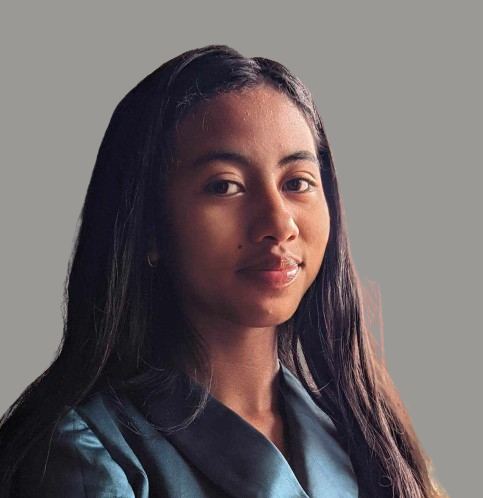
\includegraphics[width=6cm]{faniriana_cv.png} \\[0.5cm]
\end{minipage}
\hfill
\begin{minipage}{0.45\textwidth}
    \raggedright
    {\LARGE \textbf{VOAHARIMPITIAVANA}} \\[0.2cm]
    \textbf{Andraina Faniriana}\\[0.8cm]
    {\LARGE \textbf{Data analyst}}
\end{minipage}

\vspace{0.5cm}

\textbf{Profil :} \\[0.3cm]
Étudiante passionnée par l'analyse de données, motivée et autodidacte, je maîtrise les bases de la programmation et de la visualisation, avec pour objectif de contribuer à des projets concrets en tant que Data Analyste junior.\\[0.4cm]

\noindent
\begin{minipage}{0.48\textwidth}
    \raggedright
    \textbf{Contact :}
    \begin{itemize}
    \renewcommand\labelitemi{$\bullet$}
    \item \textbf{Téléphone : }0336983752
    \item \textbf{email : }andrainafaniriana@gmail.com
    \item \textbf{github : }faniriana
    \end{itemize}
    
    \vspace{0.3cm}
    \textbf{Compétences :}
    \begin{itemize}
    \renewcommand\labelitemi{$\bullet$}
    \item \textbf{Analyse de données : }Nettoyage, transformation, exploration des données
    \item \textbf{Langages : }Python (Pandas, NumPy, Matplotlib, Seaborn), SQL, R
    \item \textbf{Outils : }Excel, Power BI, Tableau, Jupyter Notebook
    \item \textbf{Base de données : }MySQL, PostgreSQL
    \item \textbf{Compétences transversales : }Rigueur, curiosité, esprit analytique, autonomie
    \end{itemize}
    
    \vspace{0.3cm}
    \textbf{Langues :}
    \begin{itemize}
    \renewcommand\labelitemi{$\bullet$}
    \item \textbf{Français : } intermédiaire
    \item \textbf{Anglais : } advanced (technical and business)
    \item \textbf{Malagasy : } langue maternelle
    \end{itemize}
\end{minipage}
\hfill
\vrule width 0.5pt
\hfill
\begin{minipage}{0.48\textwidth}
    \raggedright
    \textbf{Projets académiques et personnels :}
    \begin{itemize}
    \renewcommand\labelitemi{$\bullet$}
    \item \textbf{Analyse des facteurs associés au turnover des employés : }
        \begin{itemize}
        \renewcommand\labelitemi{$\bullet$}
            \item Dashboard turnover par département, fonction, niveau d'étude, ancienneté avec Power BI.
            \item Visualisation des départs et tendances, classification des employés
        \end{itemize}
        
    \item \textbf{Traitement de AmesHousing : }
        \begin{itemize}
        \renewcommand\labelitemi{$\bullet$}
            \item Nettoyage et normalisation des données
            \item Prédiction de prix de vente des maisons
        \end{itemize}
    \end{itemize}
    
    \vspace{0.5cm}
    \textbf{Formation :}
    \begin{itemize}
    \renewcommand\labelitemi{$\bullet$}
        \item \textbf{Licence en cours : } Université de INSI
        \item \textbf{Cours en ligne et Certifications de données en cours : } Google Cloud Skill Boost
    \end{itemize}
\end{minipage}


\newpage

% --- En-tête amélioré ---
\begin{minipage}[t]{0.18\textwidth}
  \vspace{0pt}
  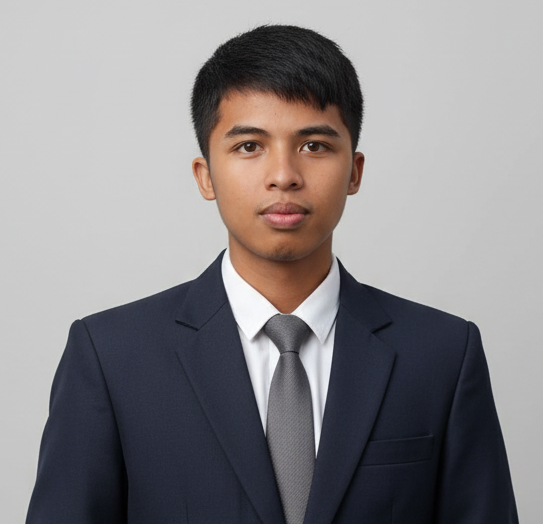
\includegraphics[width=\linewidth]{rajoCv.png}
\end{minipage}
\hfill
\begin{minipage}[t]{0.78\textwidth}
  {\Huge \textbf{\color{accentcolor} Rakotonavalona Rajo Lalaina}}\\[4pt]
  {\large \color{secondarycolor}Étudiant en Informatique – \textbf{Data Analyst Junior}}\\[8pt]
  \faIcon{map-marker-alt}\ \textcolor{accentcolor}{Antananarivo, Madagascar} \hfill
  \faIcon{envelope}\ \textcolor{accentcolor}{valkely02@gmail.com} \\[3pt]
  \faIcon{phone}\ \textcolor{accentcolor}{+261 38 98 826 79} \hfill
  \faIcon{linkedin}\ \textcolor{accentcolor}{linkedin.com/in/rajo} \\[3pt]
  \faIcon{github}\ \textcolor{accentcolor}{github.com/Naval0506}
\end{minipage}

\vspace{0.4cm}
\hrule height1.5pt
\vspace{0.4cm}

% --- Deux colonnes principales ---
\begin{minipage}[t]{0.38\textwidth}

\section*{Profil}
Étudiant passionné par l'analyse et la visualisation de données, je conçois des solutions exploitant Python, SQL et des outils BI pour transformer les données en insights exploitables. Mon objectif : participer à des projets concrets combinant technologie et impact réel.

\section*{Compétences}
\begin{skillbox}
\textbf{Analyse} : nettoyage, exploration, visualisation\\
\textbf{Langages} : Python, SQL, R\\
\textbf{Outils} : Power BI, Tableau, Excel, Jupyter\\
\textbf{ML} : régression, classification, détection d'anomalies\\
\textbf{BDD} : MySQL, PostgreSQL\\
\textbf{Soft skills} : rigueur, autonomie, curiosité
\end{skillbox}

\section*{Formation}
\textbf{Licence en Informatique (en cours)}\\
Université INSI — 2024–2025\\[4pt]
\textbf{Certifications}\\
Google Cloud Skill Boost – Data Analytics

\section*{Langues}
\begin{itemize}[leftmargin=*, label={}]
  \item \textbf{Français} : intermédiaire
  \item \textbf{Anglais} : moyen (technique)
  \item \textbf{Malagasy} : langue maternelle
\end{itemize}

\end{minipage}
\hfill
\begin{minipage}[t]{0.58\textwidth}

\section*{Projets}
\begin{itemize}[leftmargin=*, label={\color{secondarycolor}\scriptsize\faIcon{caret-right}}]
  \item \textbf{Détection de fraudes bancaires (2025)}\\
  \textit{Python, Colab, ML}\\
  Modèles supervisés (régression logistique, forêt aléatoire) pour identifier les transactions suspectes. Interface web de test et enregistrement des prédictions.
  \vspace{4pt}
  
  \item \textbf{Analyse d'habitudes d'achat (2025)}\\
  \textit{Power BI, Python}\\
  Segmentation de clients, tableaux de bord interactifs et recommandations IA pour plateforme e-commerce .
  \vspace{4pt}
  
  \item \textbf{Prédiction du prix des maisons (2024)}\\
  \textit{Ames Housing – ML}\\
  Nettoyage, normalisation et modélisation par régression (Random Forest, Linear) pour estimer les prix immobiliers.
  \vspace{4pt}
  
  \item \textbf{Gestion d'emploi du temps (2024–2025)}\\
  \textit{Symfony, MySQL}\\
  Application web pour planifier et visualiser les sessions de cours selon la semaine et la classe.
\end{itemize}

\section*{Centres d'intérêt}
\begin{itemize}[leftmargin=*, label={\color{secondarycolor}\scriptsize\faIcon{star}}]
  \item Veille technologique (IA, Data Science)
  \item Participation à des hackathons
  \item Développement de projets open source
\end{itemize}

\end{minipage}

\newpage



% ========== BIBLIOGRAPHIE ÉTENDUE ==========
\chapter*{Bibliographies}
\addcontentsline{toc}{chapter}{Bibliographie}

% === Références sur le E-commerce ===
[1] Muhammad Zusmani, \textit{Pakistan's Largest Ecommerce Dataset}, 2023, \url{https://www.kaggle.com/datasets/zusmani/pakistans-largest-ecommerce-dataset} (consulté le 27/07/2025).

[2] eMarketer, \textit{Ecommerce Growth in Africa: Trends and Forecasts 2023-2027}, 2023, \url{https://www.emarketer.com} (consulté le 05/08/2025).

[3] International Telecommunication Union, \textit{Measuring Digital Development: ICT Price Trends 2023}, 2023, \url{https://www.itu.int} (consulté le 12/07/2025).

% === Références sur le Machine Learning ===
[4] Trevor Hastie, Robert Tibshirani, Jerome Friedman, \textit{The Elements of Statistical Learning: Data Mining, Inference, and Prediction}, Springer, 2e édition, 2009. (consulté le 20/07/2025).

[5] Leo Breiman, \textit{Random Forests}, Machine Learning, vol. 45, no. 1, pp. 5–32, 2001. (consulté le 01/08/2025).

[6] Tianqi Chen, Carlos Guestrin, \textit{XGBoost: A Scalable Tree Boosting System}, Proceedings of the 22nd ACM SIGKDD, 2016. (consulté le 18/07/2025).

% === Références sur la Basket Analysis ===
[7] Rakesh Agrawal, Tomasz Imieliński, Arun Swami, \textit{Mining Association Rules Between Sets of Items in Large Databases}, Proceedings of the 1993 ACM SIGMOD, pp. 207–216, 1993. (consulté le 08/08/2025).

% === Référence académique ===
[8] Docteur ANDRIAMANJAKA RAMASONDRANO, \textit{Cours de Machine Learning}, Université INSI, Département Informatique, 2025.

\newpage
\pagestyle{plain}
\listoftables
\newpage
\pagestyle{plain}
\listoffigures
\newpage
\pagestyle{plain}
\tableofcontents
\newpage


\end{document}

